\documentclass[]{article}
\usepackage{geometry,tikz,lipsum,amsmath,amssymb,soul,xcolor,cancel,esint}
\tikzset{every picture/.style={line width=0.75pt}} %set default line width to 0.75pt        
\numberwithin{equation}{section}

\NewDocumentCommand{\caja}{ m O{gray!40} O{gray!10} m }{
	\begin{figure}[h]
		\centering
		\begin{tikzpicture}
			\node[anchor=text, text width=\columnwidth-1.2cm, draw, rounded corners, line width=1pt, fill=#3, inner sep=5mm] (big) {\\#4};
			\node[draw, rounded corners, line width=.5pt, fill=#2, anchor=west, xshift=5mm] (small) at (big.north west) {#1};
		\end{tikzpicture}
	\end{figure}
}
\NewDocumentCommand{\indUpDown}{ O{\Lambda} O{\mu} O{\nu} }{
	{#1}^{#2}_{\ #3}
}
\NewDocumentCommand{\indDownUp}{ O{\Lambda} O{\mu} O{\nu} }{
	{#1}_{#2}^{\ #3}
}
\newcommand{\LambdaMuNu}{\indUpDown}
\newcommand{\0}{\textcolor{gray}{0}}
\newcommand{\rbf}{\mathbf{r}}
\newcommand{\ei}{\mathbf{e}_i}
\newcommand{\ej}{\mathbf{e}_j}
\newcommand{\lc}{\epsilon_{ijk}}

%opening
\title{Tarea 1 Mecánica Clásica Avanzada}
\author{Simon Fonseca}

\begin{document}
\maketitle
\section{Pregunta 1}
A neutrino of the energy \(E_\nu\) scatters inelastically on a proton (\(P\)) which rests in the laboratory frame and produces a \(\pi^0\) meson with mass \(m_\pi\) and the recoil proton, via the exclusive process
\begin{equation}
	\nu + P \rightarrow \pi^0 + P'
\end{equation}
After the collision, the produced pion \(\pi^0\) and the recoil proton \(P'\) move with relativistic velocities in the laboratory frame.

% % % % % % % % % % % % % % % % % % % % % % % % % % % % % % % % % % % % % % % % % % % % % % % % % % % % % %

\begin{enumerate}
	\item[\textbf{a.}] The energy of the produced pion \(\pi^0\) in the laboratory frame is given by \(E_\pi\). The angles which form the momenta of \(\pi^0\) and recoil proton \(P'\) with the direction of neutrino beam are given by \(\theta_\nu,\theta_{P'}\). Find how the angles \(\theta_\nu,\theta_{P'}\) depend on the neutrino energy \(E_\nu\) and the pion energy \(E_\pi\).
\end{enumerate}

\begin{figure}[h!]
	\centering
	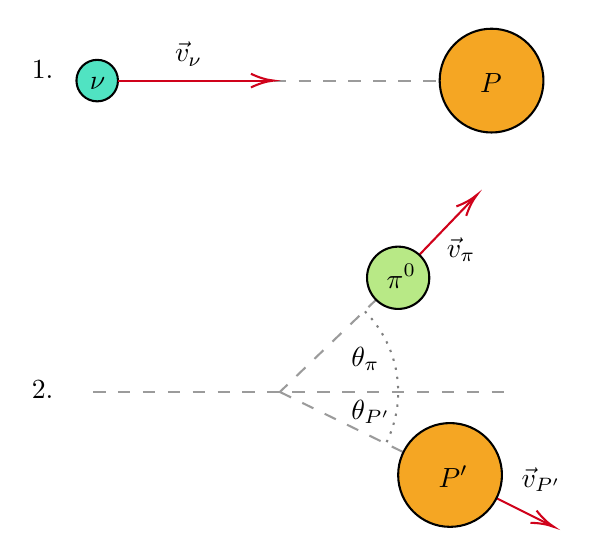
\begin{tikzpicture}[x=0.75pt,y=0.75pt,yscale=-1,xscale=1]
		%uncomment if require: \path (0,300); %set diagram left start at 0, and has height of 300
		
		%Straight Lines [id:da7616257732740312] 
		\draw [color={rgb, 255:red, 155; green, 155; blue, 155 }  ,draw opacity=1 ] [dash pattern={on 4.5pt off 4.5pt}]  (88,45) -- (238,45) ;
		%Shape: Circle [id:dp8956945294276757] 
		\draw  [fill={rgb, 255:red, 80; green, 227; blue, 194 }  ,fill opacity=1 ] (65,45) .. controls (65,39.48) and (69.48,35) .. (75,35) .. controls (80.52,35) and (85,39.48) .. (85,45) .. controls (85,50.52) and (80.52,55) .. (75,55) .. controls (69.48,55) and (65,50.52) .. (65,45) -- cycle ;
		%Shape: Circle [id:dp323687430335603] 
		\draw  [fill={rgb, 255:red, 245; green, 166; blue, 35 }  ,fill opacity=1 ] (240,45) .. controls (240,31.19) and (251.19,20) .. (265,20) .. controls (278.81,20) and (290,31.19) .. (290,45) .. controls (290,58.81) and (278.81,70) .. (265,70) .. controls (251.19,70) and (240,58.81) .. (240,45) -- cycle ;
		%Straight Lines [id:da6715018796126911] 
		\draw [color={rgb, 255:red, 208; green, 2; blue, 27 }  ,draw opacity=1 ]   (85,45) -- (158,45) ;
		\draw [shift={(160,45)}, rotate = 180] [color={rgb, 255:red, 208; green, 2; blue, 27 }  ,draw opacity=1 ][line width=0.75]    (10.93,-3.29) .. controls (6.95,-1.4) and (3.31,-0.3) .. (0,0) .. controls (3.31,0.3) and (6.95,1.4) .. (10.93,3.29)   ;
		%Straight Lines [id:da31917969652007117] 
		\draw [color={rgb, 255:red, 155; green, 155; blue, 155 }  ,draw opacity=1 ] [dash pattern={on 4.5pt off 4.5pt}]  (73,195) -- (273,195) ;
		%Straight Lines [id:da7166323914467172] 
		\draw [color={rgb, 255:red, 208; green, 2; blue, 27 }  ,draw opacity=1 ]   (210,150) -- (256.61,101.44) ;
		\draw [shift={(258,100)}, rotate = 133.83] [color={rgb, 255:red, 208; green, 2; blue, 27 }  ,draw opacity=1 ][line width=0.75]    (10.93,-3.29) .. controls (6.95,-1.4) and (3.31,-0.3) .. (0,0) .. controls (3.31,0.3) and (6.95,1.4) .. (10.93,3.29)   ;
		%Straight Lines [id:da7992423863556611] 
		\draw [color={rgb, 255:red, 155; green, 155; blue, 155 }  ,draw opacity=1 ] [dash pattern={on 4.5pt off 4.5pt}]  (210,150) -- (163,195) ;
		%Shape: Circle [id:dp4332848726531031] 
		\draw  [fill={rgb, 255:red, 184; green, 233; blue, 134 }  ,fill opacity=1 ] (205,140) .. controls (205,131.72) and (211.72,125) .. (220,125) .. controls (228.28,125) and (235,131.72) .. (235,140) .. controls (235,148.28) and (228.28,155) .. (220,155) .. controls (211.72,155) and (205,148.28) .. (205,140) -- cycle ;
		%Straight Lines [id:da8325784296854863] 
		\draw [color={rgb, 255:red, 155; green, 155; blue, 155 }  ,draw opacity=1 ] [dash pattern={on 4.5pt off 4.5pt}]  (163,195) -- (245,235) ;
		%Straight Lines [id:da35400942465013596] 
		\draw [color={rgb, 255:red, 208; green, 2; blue, 27 }  ,draw opacity=1 ]   (245,235) -- (293.21,259.11) ;
		\draw [shift={(295,260)}, rotate = 206.57] [color={rgb, 255:red, 208; green, 2; blue, 27 }  ,draw opacity=1 ][line width=0.75]    (10.93,-3.29) .. controls (6.95,-1.4) and (3.31,-0.3) .. (0,0) .. controls (3.31,0.3) and (6.95,1.4) .. (10.93,3.29)   ;
		%Shape: Circle [id:dp7327591546468705] 
		\draw  [fill={rgb, 255:red, 245; green, 166; blue, 35 }  ,fill opacity=1 ] (220,235) .. controls (220,221.19) and (231.19,210) .. (245,210) .. controls (258.81,210) and (270,221.19) .. (270,235) .. controls (270,248.81) and (258.81,260) .. (245,260) .. controls (231.19,260) and (220,248.81) .. (220,235) -- cycle ;
		%Shape: Arc [id:dp03440286807829551] 
		\draw  [draw opacity=0][dash pattern={on 0.84pt off 2.51pt}] (203.97,156.18) .. controls (213.87,166.13) and (220,179.85) .. (220,195) .. controls (220,204.15) and (217.77,212.77) .. (213.82,220.36) -- (165,195) -- cycle ; \draw  [color={rgb, 255:red, 128; green, 128; blue, 128 }  ,draw opacity=1 ][dash pattern={on 0.84pt off 2.51pt}] (203.97,156.18) .. controls (213.87,166.13) and (220,179.85) .. (220,195) .. controls (220,204.15) and (217.77,212.77) .. (213.82,220.36) ;  
		
		% Text Node
		\draw (111,25) node [anchor=north west][inner sep=0.75pt]   [align=left] {$\displaystyle \vec{v}_{\nu }$};
		% Text Node
		\draw (242,119) node [anchor=north west][inner sep=0.75pt]   [align=left] {$\displaystyle \vec{v}_{\pi }$};
		% Text Node
		\draw (278,230) node [anchor=north west][inner sep=0.75pt]   [align=left] {$\displaystyle \vec{v}_{P'}$};
		% Text Node
		\draw (196,172) node [anchor=north west][inner sep=0.75pt]   [align=left] {$\displaystyle \theta _{\pi }$};
		% Text Node
		\draw (42,34) node [anchor=north west][inner sep=0.75pt]   [align=left] {1.};
		% Text Node
		\draw (42,188) node [anchor=north west][inner sep=0.75pt]   [align=left] {2.};
		% Text Node
		\draw (70,42) node [anchor=north west][inner sep=0.75pt]    {$\nu $};
		% Text Node
		\draw (258,40) node [anchor=north west][inner sep=0.75pt]   [align=left] {$\displaystyle P$};
		% Text Node
		\draw (238,229) node [anchor=north west][inner sep=0.75pt]   [align=left] {$\displaystyle P'$};
		% Text Node
		\draw (213,132) node [anchor=north west][inner sep=0.75pt]   [align=left] {$\displaystyle \pi ^{0}$};
		% Text Node
		\draw (196,197.5) node [anchor=north west][inner sep=0.75pt]   [align=left] {$\displaystyle \theta _{P'}$};	
	\end{tikzpicture}	
\end{figure}

\textbf{NOTATION NOTE}: I'll use \(p\) and \(p^\mu\) for the 4-momentum, \(\vec{p}\) for the 3-momentum, and \(P\) for the proton label.

Taking \(c=1\). In the lab frame, rotating it for the neutrino beam to align with the \(z\) axis and the scattering plane in the \(yz\) plane:
\begin{equation}
	\begin{matrix}
		p^\mu_\nu	&=&(&E_\nu,	&\0,&\0,								&|\vec{p}_\nu|				&)\\
		p^\mu_P 	&=&(&E_P,	&\0,&\0,								&\0							&)\\
		p^\mu_\pi 	&=&(&E_\pi,	&\0,&|\vec{p}_\pi|\sin\theta_{\pi},	&|\vec{p}_\pi|\cos\theta_{\pi}&)\\
		p^\mu_{P'}	&=&(&E_{P'},&\0,&-|\vec{p}_{P'}|\sin\theta_{P'},	&|\vec{p}_{P'}|\cos\theta_{P'}&)
	\end{matrix}
\end{equation}
But, because of \textit{on-shell} conditions:
\begin{align}
	E_\nu &\approx |\vec{p}_\nu|\label{Enu_equiv}\\
	E_P &= m_P\label{EP_equiv}\\
	E_\pi &= \sqrt{\vec{p}_\pi^2 + m_\pi^2}\label{Epi_equiv}\\
	E_{P'} &= \sqrt{\vec{p}_{P'}^2 + m_P^2}\label{EP'_equiv}
\end{align}
\begin{align}
	\Rightarrow |\vec{p}_\pi|  &= \sqrt{E_\pi^2  - m_\pi^2}\label{ppi_equiv}\\
	\Rightarrow |\vec{p}_{P'}| &= \sqrt{E_{P'}^2 - m_P^2}\label{pp'_equiv}
\end{align}
And the  conservation of energy-momentum:
\begin{equation}
	p^\mu_\nu + p^\mu_P = p^\mu_\pi + p^\mu_{P'}\label{cons_EM}
%	0 &= |\vec{p}_\pi|\sin\theta_{\pi} - |\vec{p}_{P'}|\sin\theta_{P'}\\
%	p_\nu &= |\vec{p}_\pi|\cos\theta_{\pi} + |\vec{p}_{P'}|\cos\theta_{P'}
\end{equation}
\begin{align}
	E_\nu + E_P &= E_\pi + E_{P'}\nonumber\\
	\Rightarrow E_{P'} &= E_\nu + E_P - E_\pi\label{EP'_cons_E}
\end{align}
%\begin{align}
%	\Rightarrow E_{p'} &= E_\nu + m_p - E_{\pi}\\
%	\Rightarrow |\vec{p}_{p'}| &= \sqrt{(E_\nu - E_{\pi})}\cdot\sqrt{(E_\nu + 2 m_p - E_{\pi})}
%\end{align}
From eq. \ref{cons_EM}:
\begin{align*}
	p^\mu_{P'} &= p^\mu_\nu + p^\mu_P - p^\mu_\pi\\
	\Rightarrow (p^\mu_{P'})^2 &= (p^\mu_\nu + p^\mu_P - p^\mu_\pi)^2
\end{align*}
but \((p^\mu)^2 = p^2 = p^\mu p_\nu = m^2\), so
\begin{align*}
	\Rightarrow p_{P'}^2 &= p_\nu^2 + p_P^2 + p_\pi^2 + \textcolor{red}{(p_\nu)^\lambda (p_P)_\lambda} - \textcolor{blue}{(p_\nu)^\alpha (p_\pi)_\alpha} - \textcolor{purple}{(p_P)^\beta (p_\pi)_\beta}\\
	\Rightarrow \cancel{m_P^2} &= \cancel{m_\nu^2} + \cancel{m_p^2} + m_\pi^2 +\textcolor{red}{2 E_P E_\nu} - \textcolor{blue}{2(E_\nu E_\pi - |\vec{p}_\nu| |\vec{p}_\pi|\cos\theta_{\pi})} - \textcolor{purple}{2E_P E_\pi}
\end{align*}
solving for \(\cos\theta_\pi\), using equations \ref{Enu_equiv}, \ref{EP_equiv} and \ref{ppi_equiv}:
\begin{align*}
	2 E_\nu \sqrt{E_\pi^2  - m_\pi^2} \cos\theta_\pi &= - m_\pi^2 - 2m_P E_\nu + 2E_\nu E_\pi + 2m_P E_\pi\\
	\Rightarrow \cos\theta_\pi &= \frac{- m_\pi^2 - 2m_P E_\nu + 2E_\nu E_\pi + 2m_P E_\pi}{2 E_\nu \sqrt{E_\pi^2  - m_\pi^2} }
\end{align*}
From eq. \ref{cons_EM}:
\begin{align*}
p^\mu_\pi &= p^\mu_\nu + p^\mu_P - p^\mu_{P'}\\
\Rightarrow (p^\mu_\pi)^2 &= (p^\mu_\nu + p^\mu_P - p^\mu_{P'})^2
\end{align*}
\begin{align*}
\Rightarrow p_\pi^2 &= p_\nu^2 + p_P^2 + p_{P'}^2 + \textcolor{red}{(p_\nu)^\lambda (p_P)_\lambda} - \textcolor{blue}{(p_\nu)^\alpha (p_{P'})_\alpha} - \textcolor{purple}{(p_P)^\beta (p_{P'})_\beta}\\
\Rightarrow m_\pi^2 &= \cancel{m_\nu^2} + m_P^2 + m_P^2 +\textcolor{red}{2 E_P E_\nu} - \textcolor{blue}{2(E_\nu E_{P'} - |\vec{p}_\nu| |\vec{p}_{P'}|\cos\theta_{P'})} - \textcolor{purple}{2 E_P E_{P'}}
\end{align*}
solving for \(\cos\theta_{P'}\), using equations \ref{Enu_equiv}, \ref{EP_equiv}, \ref{pp'_equiv} and \ref{EP'_cons_E}:
\begin{align*}
0 &= 2m_P^2 - m_\pi^2 + 2 m_P E_\nu - 2 E_\nu E_{P'} + 2 E_\nu \sqrt{E_{P'}^2 - m_P^2} \cos\theta_{P'} - 2 m_P E_{P'}\\
2 E_\nu \sqrt{E_{P'}^2 - m_P^2} \cos\theta_{P'} &= - 2 m_P^2 + m_\pi^2 - 2 m_P E_\nu + 2 E_\nu (E_\nu + m_P - E_\pi) + 2 m_P (E_\nu + m_P - E_\pi)
\end{align*}
\begin{align*}
	\cos\theta_{P'} = \frac{2 (E_\nu - E_\pi) (E_\nu + m_P) + m_\pi^2}{2 E_\nu \sqrt{(E_\nu - E_\pi) (E_\nu - E_\pi + 2 m_P)}}
\end{align*}

Finally:
\begin{equation}
	\left\lbrace \begin{matrix}
		\theta_\pi(E_\nu, E_\pi)  &=& \arccos\left( \dfrac{- m_\pi^2 - 2m_P E_\nu + 2E_\nu E_\pi + 2m_P E_\pi}{2 E_\nu \sqrt{E_\pi^2  - m_\pi^2} }\right)\vspace{5mm}\\
		\theta_{P'}(E_\nu, E_\pi) &=& \arccos\left( \dfrac{2 (E_\nu - E_\pi) (E_\nu + m_P) + m_\pi^2}{2 E_\nu \sqrt{(E_\nu - E_\pi) (E_\nu - E_\pi + 2 m_P)}}\right) 
	\end{matrix}\right.
	\label{angulos_EnuEpi}
\end{equation}
And all the 4-momentums written as functions of \(E_\nu,E_\pi\) and constant parameters is
\begin{equation}
	\begin{matrix}
		p^\mu_\nu	&=&(&E_\nu,	&\0,&\0,								&E_\nu				&)\\
		p^\mu_P 	&=&(&m_P,	&\0,&\0,								&\0							&)\\
		p^\mu_\pi 	&=&(&E_\pi,	&\0,&|\vec{p}_\pi|\sin\theta_{\pi},	&|\vec{p}_\pi|\cos\theta_{\pi}&)\\
		p^\mu_{P'}	&=&(&E_\nu - E_\pi + m_P,&\0,&-|\vec{p}_{P'}|\sin\theta_{P'},	&|\vec{p}_{P'}|\cos\theta_{P'}&)
	\end{matrix}
	\label{momentums_EnuEpi}
\end{equation}
where
\begin{equation}
	\begin{matrix}
		|\vec{p}_\pi| = \sqrt{E_\pi^2  - m_\pi^2},& |\vec{p}_{P'}| = \sqrt{(E_\nu-E_\pi) (E_\nu - E_\pi + 2 m_P)}
	\end{matrix}
	\label{ppi_pp'_EnuEpi}
\end{equation}
\\
% % % % % % % % % % % % % % % % % % % % % % % % % % % % % % % % % % % % % % % % % % % % % % % % % % % % % %

\begin{enumerate}
	\item[\textbf{b.}] Write out explicit expressions for the Mandelstam variables \(s, t, u\) in terms of the energy of the incoming neutrino \(E_\nu\) and the energy of pion \(E_\pi\) defined in the previous item.
\end{enumerate}

The Mandelstam variables:
\begin{alignat}{2}
	s &= (p_\nu + p_P)^2 &&= (p_\pi + p_{P'})^2\\
	t &= (p_P - p_{P'})^2 &&= (p_\nu - p_\pi)^2\\
	u &= (p_\nu - p_{P'})^2 &&= (p_P - p_\pi)^2
\end{alignat}

Choosing the more convenient equivalencies, using equations \ref{angulos_EnuEpi}, \ref{momentums_EnuEpi}, \ref{ppi_pp'_EnuEpi}:
\begin{align}
	s &= (p_\nu + p_P)^2\nonumber\\
	s &= \cancel{p_\nu^2} + 2 p_\nu p_P + p_P^2\nonumber\\
	s &= 0 + 2 E_\nu E_P + m_P^2\nonumber\\
	\Rightarrow s &= 2 m_P E_\nu + m_P^2\\\nonumber\\
	t &= (p_P - p_{P'})^2\nonumber\\
	t &= p_P^2 - 2 p_P p_{P'} + p_{P'}^2\nonumber\\
	t &= m_P^2 - 2 m_P (E_\nu - E_\pi + m_P) + m_P^2\nonumber\\
	\Rightarrow t &= 2 m_P E_\pi - 2 m_P E_\nu\\\nonumber\\
	u &= (p_P - p_\pi)^2\nonumber\\
	u &= p_P^2 - 2 p_P p_\pi + p_\pi^2\nonumber\\
	\Rightarrow u &= m_P^2 - 2 m_P E_\pi + m_\pi^2
\end{align}

It's easy to show that:
\begin{equation}
	s + t + u = 2 m_P^2 + m_\pi^2
\end{equation}
\\
% % % % % % % % % % % % % % % % % % % % % % % % % % % % % % % % % % % % % % % % % % % % % % % % % % % % % %

\begin{enumerate}
\item[\textbf{c.}] Find the minimal energy \(E^\text{(min)}_\nu\) of the neutrino may lead to the pion production.
\end{enumerate}
If we do a Lorentz boost to the CM-frame so that the sum of the momentum before and after the collision is net zero, and we redefine the angles of scattering we get

\begin{figure}[h!]
	\centering
	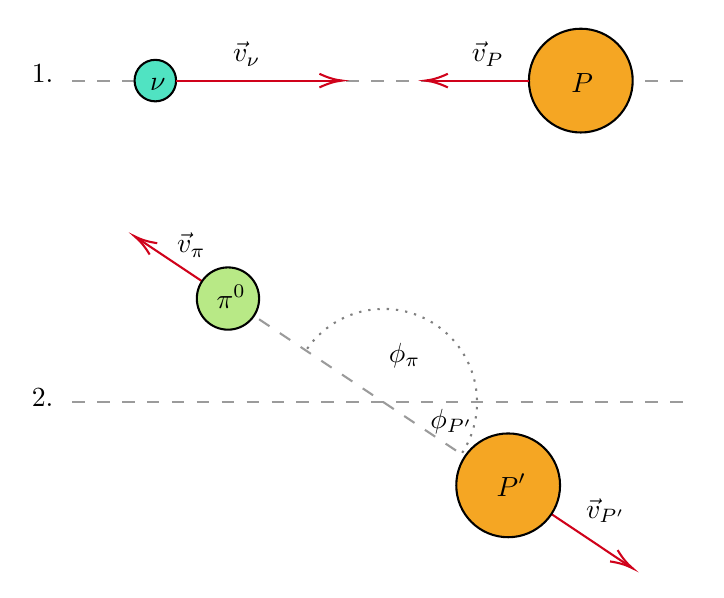
\begin{tikzpicture}[x=0.75pt,y=0.75pt,yscale=-1,xscale=1]
			%uncomment if require: \path (0,300); %set diagram left start at 0, and has height of 300
			
			%Shape: Boxed Line [id:dp3768023523094234] 
			\draw [color={rgb, 255:red, 155; green, 155; blue, 155 }  ,draw opacity=1 ] [dash pattern={on 4.5pt off 4.5pt}]  (60,195) -- (360,195) ;
			%Straight Lines [id:da9567812381434895] 
			\draw [color={rgb, 255:red, 208; green, 2; blue, 27 }  ,draw opacity=1 ]   (135,145) -- (91.66,116.11) ;
			\draw [shift={(90,115)}, rotate = 33.69] [color={rgb, 255:red, 208; green, 2; blue, 27 }  ,draw opacity=1 ][line width=0.75]    (10.93,-3.29) .. controls (6.95,-1.4) and (3.31,-0.3) .. (0,0) .. controls (3.31,0.3) and (6.95,1.4) .. (10.93,3.29)   ;
			%Shape: Circle [id:dp2755889008931569] 
			\draw  [fill={rgb, 255:red, 184; green, 233; blue, 134 }  ,fill opacity=1 ] (120,145) .. controls (120,136.72) and (126.72,130) .. (135,130) .. controls (143.28,130) and (150,136.72) .. (150,145) .. controls (150,153.28) and (143.28,160) .. (135,160) .. controls (126.72,160) and (120,153.28) .. (120,145) -- cycle ;
			
			%Shape: Boxed Line [id:dp7352039641203345] 
			\draw [color={rgb, 255:red, 155; green, 155; blue, 155 }  ,draw opacity=1 ] [dash pattern={on 4.5pt off 4.5pt}]  (150,155) -- (270,235) ;
			%Straight Lines [id:da9617978862938473] 
			\draw [color={rgb, 255:red, 208; green, 2; blue, 27 }  ,draw opacity=1 ]   (285.48,245.24) -- (328.34,273.89) ;
			\draw [shift={(330,275)}, rotate = 213.76] [color={rgb, 255:red, 208; green, 2; blue, 27 }  ,draw opacity=1 ][line width=0.75]    (10.93,-3.29) .. controls (6.95,-1.4) and (3.31,-0.3) .. (0,0) .. controls (3.31,0.3) and (6.95,1.4) .. (10.93,3.29)   ;
			%Shape: Arc [id:dp16255090776029524] 
			\draw  [draw opacity=0][dash pattern={on 0.84pt off 2.51pt}] (173.14,169.19) .. controls (181.27,157.58) and (194.75,150) .. (210,150) .. controls (234.85,150) and (255,170.15) .. (255,195) .. controls (255,204.6) and (251.99,213.51) .. (246.86,220.81) -- (210,195) -- cycle ; \draw  [color={rgb, 255:red, 128; green, 128; blue, 128 }  ,draw opacity=1 ][dash pattern={on 0.84pt off 2.51pt}] (173.14,169.19) .. controls (181.27,157.58) and (194.75,150) .. (210,150) .. controls (234.85,150) and (255,170.15) .. (255,195) .. controls (255,204.6) and (251.99,213.51) .. (246.86,220.81) ;  
			%Straight Lines [id:da4881285644911042] 
			\draw [color={rgb, 255:red, 155; green, 155; blue, 155 }  ,draw opacity=1 ] [dash pattern={on 4.5pt off 4.5pt}]  (60,40) -- (360,40) ;
			%Shape: Circle [id:dp148514510808456] 
			\draw  [fill={rgb, 255:red, 80; green, 227; blue, 194 }  ,fill opacity=1 ] (90,40) .. controls (90,34.48) and (94.48,30) .. (100,30) .. controls (105.52,30) and (110,34.48) .. (110,40) .. controls (110,45.52) and (105.52,50) .. (100,50) .. controls (94.48,50) and (90,45.52) .. (90,40) -- cycle ;
			%Shape: Circle [id:dp23403725209220883] 
			\draw  [fill={rgb, 255:red, 245; green, 166; blue, 35 }  ,fill opacity=1 ] (280,40) .. controls (280,26.19) and (291.19,15) .. (305,15) .. controls (318.81,15) and (330,26.19) .. (330,40) .. controls (330,53.81) and (318.81,65) .. (305,65) .. controls (291.19,65) and (280,53.81) .. (280,40) -- cycle ;
			%Straight Lines [id:da1387036169563105] 
			\draw [color={rgb, 255:red, 208; green, 2; blue, 27 }  ,draw opacity=1 ]   (110,40) -- (188,40) ;
			\draw [shift={(190,40)}, rotate = 180] [color={rgb, 255:red, 208; green, 2; blue, 27 }  ,draw opacity=1 ][line width=0.75]    (10.93,-3.29) .. controls (6.95,-1.4) and (3.31,-0.3) .. (0,0) .. controls (3.31,0.3) and (6.95,1.4) .. (10.93,3.29)   ;
			%Straight Lines [id:da6486578531409215] 
			\draw [color={rgb, 255:red, 208; green, 2; blue, 27 }  ,draw opacity=1 ]   (280,40) -- (232,40) ;
			\draw [shift={(230,40)}, rotate = 360] [color={rgb, 255:red, 208; green, 2; blue, 27 }  ,draw opacity=1 ][line width=0.75]    (10.93,-3.29) .. controls (6.95,-1.4) and (3.31,-0.3) .. (0,0) .. controls (3.31,0.3) and (6.95,1.4) .. (10.93,3.29)   ;
			%Shape: Circle [id:dp8819611394623612] 
			\draw  [fill={rgb, 255:red, 245; green, 166; blue, 35 }  ,fill opacity=1 ] (245,235) .. controls (245,221.19) and (256.19,210) .. (270,210) .. controls (283.81,210) and (295,221.19) .. (295,235) .. controls (295,248.81) and (283.81,260) .. (270,260) .. controls (256.19,260) and (245,248.81) .. (245,235) -- cycle ;
			
			% Text Node
			\draw (109,112) node [anchor=north west][inner sep=0.75pt]   [align=left] {$\displaystyle \vec{v}_{\pi }$};
			% Text Node
			\draw (306,240) node [anchor=north west][inner sep=0.75pt]   [align=left] {$\displaystyle \vec{v}_{P'}$};
			% Text Node
			\draw (211,165) node [anchor=north west][inner sep=0.75pt]   [align=left] {$\displaystyle \phi _{\pi }$};
			% Text Node
			\draw (39,187) node [anchor=north west][inner sep=0.75pt]   [align=left] {2.};
			% Text Node
			\draw (231,197) node [anchor=north west][inner sep=0.75pt]   [align=left] {$\displaystyle \phi _{P'}$};
			% Text Node
			\draw (136,20) node [anchor=north west][inner sep=0.75pt]   [align=left] {$\displaystyle \vec{v}_{\nu }$};
			% Text Node
			\draw (39,31) node [anchor=north west][inner sep=0.75pt]   [align=left] {1.};
			% Text Node
			\draw (96,37.4) node [anchor=north west][inner sep=0.75pt]    {$\nu $};
			% Text Node
			\draw (299,35) node [anchor=north west][inner sep=0.75pt]   [align=left] {$\displaystyle P$};
			% Text Node
			\draw (251,20) node [anchor=north west][inner sep=0.75pt]   [align=left] {$\displaystyle \vec{v}_{P}$};
			% Text Node
			\draw (128,137) node [anchor=north west][inner sep=0.75pt]   [align=left] {$\displaystyle \pi ^{0}$};
			% Text Node
			\draw (263,228) node [anchor=north west][inner sep=0.75pt]   [align=left] {$\displaystyle P'$};
			
			
		\end{tikzpicture}
\end{figure}

\begin{equation}
	\begin{matrix}
			p^\mu_\nu	&= &(E_\nu,		&\0, &\0, 							&|\vec{p}_\text{i}|)\\
			p^\mu_P 	&= &(E_P,		&\0, &\0,							&-|\vec{p}_\text{i}|)\\
			p^\mu_\pi 	&= &(E_\pi,		&\0, &|\vec{p}_\pi|\sin\phi_{\pi},	&|\vec{p}_\pi|\cos\phi_{\pi})\\
			p^\mu_{P'}	&= &(E_{P'},	&\0, &-|\vec{p}_{P'}|\sin\phi_{P'},	&|\vec{p}_{P'}|\cos\phi_{P'})
		\end{matrix}
\end{equation}
where \(|\vec{p}_\text{i}|\) is the magnitude of the initial momentum, so that
\begin{equation}
	\vec{p}_\nu + \vec{p}_P = |\vec{p}_\text{i}| - |\vec{p}_\text{i}| = \vec{0}
\end{equation}
Then, because of the condition of \textit{on shell} mass:
\begin{align}
	p_\nu^2 = E_\nu^2 - p_\text{i}^2 &= m_\nu^2 \approx 0\nonumber\\
	\Rightarrow p_\text{i} &\approx E_\nu\label{pi_Enu}\\
	p_P^2 = E_P^2 - p_\text{i}^2 &= m_P^2\nonumber\\
	\Rightarrow E_P &\approx \sqrt{m_P^2 + E_\nu^2}\label{EP}
\end{align}
Then, because of conservation of energy, and using equations \ref{Epi_equiv} and \ref{EP'_equiv}:
\begin{align*}
	E_\nu + E_P &= E_{P'} + E_\pi\\
	\Rightarrow E_\nu + \sqrt{m_P^2 + E_\nu^2} &= \sqrt{\vec{p}_\pi^2 + m_\pi^2} + \sqrt{\vec{p}_{P'}^2 + m_P^2}
\end{align*}
The minimum \(E_\nu\) energy will be the one that reduces to zero the momentum of the outgoing particles, leaving only the barebone mass parameters:
\begin{equation*}
	\begin{matrix}
		\vec{p}_\pi = 0,& \vec{p}_{P'} = 0
	\end{matrix}
\end{equation*}
\begin{equation*}
	\Rightarrow E^\text{(min)}_\nu + \sqrt{m_P^2 + \left(E^\text{(min)}_\nu\right)^2} = m_\pi + m_P
\end{equation*}
Solving for \(E^\text{(min)}_\nu\):
\begin{equation}
	E^\text{(min)}_\nu = \frac{m_\pi (m_\pi + 2 m_P)}{2 (m_\pi + m_P)}
\end{equation}

%%%%%%%%%%%%%%%%%%%%%%%%%%%%%%%%%%%%%%%%%%%%%%%%%%%%%%%%%%%%%%%%%%%%%%%%%%%%%%%%%%%%%%%%%%%%%%%%%%%%%%%%%%%

\section{Pregunta 2}
A relativistic particle of mass \(m\) and electric charge \(q\) moves in a constant homogeneous electromagnetic field in which the electric field \(\mathbf{E}\) is perpendicular to the magnetic field \(\mathbf{B}\) and \(|\mathbf{E}| = c|\mathbf{B}|\). The initial velocity of particle \(\mathbf{v}\) is perpendicular to both \(\mathbf{E}\) and \(\mathbf{B} \).

% % % % % % % % % % % % % % % % % % % % % % % % % % % % % % % % % % % % % % % % % % % % % % % % % % % % % %

\begin{enumerate}
	\item[\textbf{a.}] Write out the equations of motion and find the trajectory of the particle in this field.
\end{enumerate}

Choosing:
\begin{align}
	\mathbf{p} &= \mathbf{p}(t)\\
	\mathbf{E} &= c B \hat{\mathbf{y}}\label{Ecampo}\\
	\mathbf{B} &= B \hat{\mathbf{z}}
\end{align}
With 
\begin{equation}
	\mathbf{p}(t = 0) = p_{0x} \hat{\mathbf{x}}\label{p_0}
\end{equation}
\begin{figure}[h!]
	\centering
	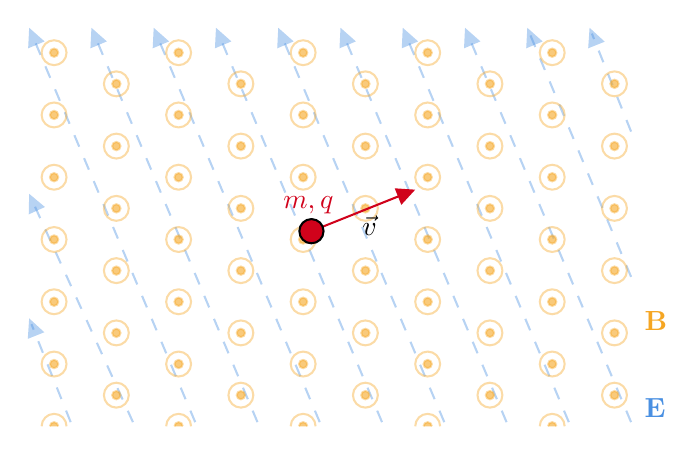
\begin{tikzpicture}[x=0.75pt,y=0.75pt,yscale=-1,xscale=1]
		%uncomment if require: \path (0,300); %set diagram left start at 0, and has height of 300
		
		%Straight Lines [id:da3451932225892893] 
		\draw [color={rgb, 255:red, 74; green, 144; blue, 226 }  ,draw opacity=0.4 ] [dash pattern={on 4.5pt off 4.5pt}]  (326,211) -- (247.16,23.76) ;
		\draw [shift={(246,21)}, rotate = 67.17] [fill={rgb, 255:red, 74; green, 144; blue, 226 }  ,fill opacity=0.4 ][line width=0.08]  [draw opacity=0] (8.93,-4.29) -- (0,0) -- (8.93,4.29) -- cycle    ;
		%Straight Lines [id:da013890970875816144] 
		\draw [color={rgb, 255:red, 74; green, 144; blue, 226 }  ,draw opacity=0.4 ] [dash pattern={on 4.5pt off 4.5pt}]  (296,211) -- (217.16,23.76) ;
		\draw [shift={(216,21)}, rotate = 67.17] [fill={rgb, 255:red, 74; green, 144; blue, 226 }  ,fill opacity=0.4 ][line width=0.08]  [draw opacity=0] (8.93,-4.29) -- (0,0) -- (8.93,4.29) -- cycle    ;
		%Straight Lines [id:da049680223944745694] 
		\draw [color={rgb, 255:red, 74; green, 144; blue, 226 }  ,draw opacity=0.4 ] [dash pattern={on 4.5pt off 4.5pt}]  (266,211) -- (187.16,23.76) ;
		\draw [shift={(186,21)}, rotate = 67.17] [fill={rgb, 255:red, 74; green, 144; blue, 226 }  ,fill opacity=0.4 ][line width=0.08]  [draw opacity=0] (8.93,-4.29) -- (0,0) -- (8.93,4.29) -- cycle    ;
		%Straight Lines [id:da18098658688735902] 
		\draw [color={rgb, 255:red, 74; green, 144; blue, 226 }  ,draw opacity=0.4 ] [dash pattern={on 4.5pt off 4.5pt}]  (236,211) -- (157.16,23.76) ;
		\draw [shift={(156,21)}, rotate = 67.17] [fill={rgb, 255:red, 74; green, 144; blue, 226 }  ,fill opacity=0.4 ][line width=0.08]  [draw opacity=0] (8.93,-4.29) -- (0,0) -- (8.93,4.29) -- cycle    ;
		%Straight Lines [id:da08641158054744891] 
		\draw [color={rgb, 255:red, 74; green, 144; blue, 226 }  ,draw opacity=0.4 ] [dash pattern={on 4.5pt off 4.5pt}]  (206,211) -- (127.16,23.76) ;
		\draw [shift={(126,21)}, rotate = 67.17] [fill={rgb, 255:red, 74; green, 144; blue, 226 }  ,fill opacity=0.4 ][line width=0.08]  [draw opacity=0] (8.93,-4.29) -- (0,0) -- (8.93,4.29) -- cycle    ;
		%Straight Lines [id:da4418290141727912] 
		\draw [color={rgb, 255:red, 74; green, 144; blue, 226 }  ,draw opacity=0.4 ] [dash pattern={on 4.5pt off 4.5pt}]  (176,211) -- (97.16,23.76) ;
		\draw [shift={(96,21)}, rotate = 67.17] [fill={rgb, 255:red, 74; green, 144; blue, 226 }  ,fill opacity=0.4 ][line width=0.08]  [draw opacity=0] (8.93,-4.29) -- (0,0) -- (8.93,4.29) -- cycle    ;
		%Straight Lines [id:da72639553864311] 
		\draw [color={rgb, 255:red, 74; green, 144; blue, 226 }  ,draw opacity=0.4 ] [dash pattern={on 4.5pt off 4.5pt}]  (146,211) -- (67.16,23.76) ;
		\draw [shift={(66,21)}, rotate = 67.17] [fill={rgb, 255:red, 74; green, 144; blue, 226 }  ,fill opacity=0.4 ][line width=0.08]  [draw opacity=0] (8.93,-4.29) -- (0,0) -- (8.93,4.29) -- cycle    ;
		%Straight Lines [id:da4477547941011977] 
		\draw [color={rgb, 255:red, 74; green, 144; blue, 226 }  ,draw opacity=0.4 ] [dash pattern={on 4.5pt off 4.5pt}]  (326,141) -- (277.15,23.77) ;
		\draw [shift={(276,21)}, rotate = 67.38] [fill={rgb, 255:red, 74; green, 144; blue, 226 }  ,fill opacity=0.4 ][line width=0.08]  [draw opacity=0] (8.93,-4.29) -- (0,0) -- (8.93,4.29) -- cycle    ;
		%Straight Lines [id:da29906011381419084] 
		\draw [color={rgb, 255:red, 74; green, 144; blue, 226 }  ,draw opacity=0.4 ] [dash pattern={on 4.5pt off 4.5pt}]  (116,211) -- (37.16,23.76) ;
		\draw [shift={(36,21)}, rotate = 67.17] [fill={rgb, 255:red, 74; green, 144; blue, 226 }  ,fill opacity=0.4 ][line width=0.08]  [draw opacity=0] (8.93,-4.29) -- (0,0) -- (8.93,4.29) -- cycle    ;
		%Straight Lines [id:da29271505832951905] 
		\draw [color={rgb, 255:red, 74; green, 144; blue, 226 }  ,draw opacity=0.4 ] [dash pattern={on 4.5pt off 4.5pt}]  (86,211) -- (37.24,103.73) ;
		\draw [shift={(36,101)}, rotate = 65.56] [fill={rgb, 255:red, 74; green, 144; blue, 226 }  ,fill opacity=0.4 ][line width=0.08]  [draw opacity=0] (8.93,-4.29) -- (0,0) -- (8.93,4.29) -- cycle    ;
		%Straight Lines [id:da5559230943014137] 
		\draw [color={rgb, 255:red, 74; green, 144; blue, 226 }  ,draw opacity=0.4 ] [dash pattern={on 4.5pt off 4.5pt}]  (326,71) -- (307.11,23.79) ;
		\draw [shift={(306,21)}, rotate = 68.2] [fill={rgb, 255:red, 74; green, 144; blue, 226 }  ,fill opacity=0.4 ][line width=0.08]  [draw opacity=0] (8.93,-4.29) -- (0,0) -- (8.93,4.29) -- cycle    ;
		%Straight Lines [id:da1113818198524501] 
		\draw [color={rgb, 255:red, 74; green, 144; blue, 226 }  ,draw opacity=0.4 ] [dash pattern={on 4.5pt off 4.5pt}]  (56,211) -- (37.11,163.79) ;
		\draw [shift={(36,161)}, rotate = 68.2] [fill={rgb, 255:red, 74; green, 144; blue, 226 }  ,fill opacity=0.4 ][line width=0.08]  [draw opacity=0] (8.93,-4.29) -- (0,0) -- (8.93,4.29) -- cycle    ;
		
		%Shape: Circle [id:dp31131058304766923] 
		\draw  [color={rgb, 255:red, 245; green, 166; blue, 35 }  ,draw opacity=0.4 ] (324,198) .. controls (324,201.31) and (321.31,204) .. (318,204) .. controls (314.69,204) and (312,201.31) .. (312,198) .. controls (312,194.69) and (314.69,192) .. (318,192) .. controls (321.31,192) and (324,194.69) .. (324,198) -- cycle ;
		%Shape: Ellipse [id:dp14495718884868758] 
		\draw  [color={rgb, 255:red, 245; green, 166; blue, 35 }  ,draw opacity=0.4 ][fill={rgb, 255:red, 245; green, 166; blue, 35 }  ,fill opacity=0.6 ] (316,198) .. controls (316,199.1) and (316.9,200) .. (318,200) .. controls (319.1,200) and (320,199.1) .. (320,198) .. controls (320,196.9) and (319.1,196) .. (318,196) .. controls (316.9,196) and (316,196.9) .. (316,198) -- cycle ;
		
		%Shape: Circle [id:dp6880480046786177] 
		\draw  [color={rgb, 255:red, 245; green, 166; blue, 35 }  ,draw opacity=0.4 ] (324,168) .. controls (324,171.31) and (321.31,174) .. (318,174) .. controls (314.69,174) and (312,171.31) .. (312,168) .. controls (312,164.69) and (314.69,162) .. (318,162) .. controls (321.31,162) and (324,164.69) .. (324,168) -- cycle ;
		%Shape: Ellipse [id:dp9882747859072925] 
		\draw  [color={rgb, 255:red, 245; green, 166; blue, 35 }  ,draw opacity=0.4 ][fill={rgb, 255:red, 245; green, 166; blue, 35 }  ,fill opacity=0.6 ] (316,168) .. controls (316,169.1) and (316.9,170) .. (318,170) .. controls (319.1,170) and (320,169.1) .. (320,168) .. controls (320,166.9) and (319.1,166) .. (318,166) .. controls (316.9,166) and (316,166.9) .. (316,168) -- cycle ;
		
		%Shape: Circle [id:dp6261435727988145] 
		\draw  [color={rgb, 255:red, 245; green, 166; blue, 35 }  ,draw opacity=0.4 ] (324,138) .. controls (324,141.31) and (321.31,144) .. (318,144) .. controls (314.69,144) and (312,141.31) .. (312,138) .. controls (312,134.69) and (314.69,132) .. (318,132) .. controls (321.31,132) and (324,134.69) .. (324,138) -- cycle ;
		%Shape: Ellipse [id:dp6730625715222709] 
		\draw  [color={rgb, 255:red, 245; green, 166; blue, 35 }  ,draw opacity=0.4 ][fill={rgb, 255:red, 245; green, 166; blue, 35 }  ,fill opacity=0.6 ] (316,138) .. controls (316,139.1) and (316.9,140) .. (318,140) .. controls (319.1,140) and (320,139.1) .. (320,138) .. controls (320,136.9) and (319.1,136) .. (318,136) .. controls (316.9,136) and (316,136.9) .. (316,138) -- cycle ;
		
		%Shape: Circle [id:dp14134704508626894] 
		\draw  [color={rgb, 255:red, 245; green, 166; blue, 35 }  ,draw opacity=0.4 ] (324,108) .. controls (324,111.31) and (321.31,114) .. (318,114) .. controls (314.69,114) and (312,111.31) .. (312,108) .. controls (312,104.69) and (314.69,102) .. (318,102) .. controls (321.31,102) and (324,104.69) .. (324,108) -- cycle ;
		%Shape: Ellipse [id:dp29119570695202435] 
		\draw  [color={rgb, 255:red, 245; green, 166; blue, 35 }  ,draw opacity=0.4 ][fill={rgb, 255:red, 245; green, 166; blue, 35 }  ,fill opacity=0.6 ] (316,108) .. controls (316,109.1) and (316.9,110) .. (318,110) .. controls (319.1,110) and (320,109.1) .. (320,108) .. controls (320,106.9) and (319.1,106) .. (318,106) .. controls (316.9,106) and (316,106.9) .. (316,108) -- cycle ;
		
		%Shape: Circle [id:dp23665416830902308] 
		\draw  [color={rgb, 255:red, 245; green, 166; blue, 35 }  ,draw opacity=0.4 ] (324,78) .. controls (324,81.31) and (321.31,84) .. (318,84) .. controls (314.69,84) and (312,81.31) .. (312,78) .. controls (312,74.69) and (314.69,72) .. (318,72) .. controls (321.31,72) and (324,74.69) .. (324,78) -- cycle ;
		%Shape: Ellipse [id:dp5450108377287437] 
		\draw  [color={rgb, 255:red, 245; green, 166; blue, 35 }  ,draw opacity=0.4 ][fill={rgb, 255:red, 245; green, 166; blue, 35 }  ,fill opacity=0.6 ] (316,78) .. controls (316,79.1) and (316.9,80) .. (318,80) .. controls (319.1,80) and (320,79.1) .. (320,78) .. controls (320,76.9) and (319.1,76) .. (318,76) .. controls (316.9,76) and (316,76.9) .. (316,78) -- cycle ;
		
		%Shape: Circle [id:dp10686308922541055] 
		\draw  [color={rgb, 255:red, 245; green, 166; blue, 35 }  ,draw opacity=0.4 ] (324,48) .. controls (324,51.31) and (321.31,54) .. (318,54) .. controls (314.69,54) and (312,51.31) .. (312,48) .. controls (312,44.69) and (314.69,42) .. (318,42) .. controls (321.31,42) and (324,44.69) .. (324,48) -- cycle ;
		%Shape: Ellipse [id:dp6449715091465903] 
		\draw  [color={rgb, 255:red, 245; green, 166; blue, 35 }  ,draw opacity=0.4 ][fill={rgb, 255:red, 245; green, 166; blue, 35 }  ,fill opacity=0.6 ] (316,48) .. controls (316,49.1) and (316.9,50) .. (318,50) .. controls (319.1,50) and (320,49.1) .. (320,48) .. controls (320,46.9) and (319.1,46) .. (318,46) .. controls (316.9,46) and (316,46.9) .. (316,48) -- cycle ;
		
		%Shape: Circle [id:dp7022144617142049] 
		\draw  [color={rgb, 255:red, 245; green, 166; blue, 35 }  ,draw opacity=0.4 ] (294,183) .. controls (294,186.31) and (291.31,189) .. (288,189) .. controls (284.69,189) and (282,186.31) .. (282,183) .. controls (282,179.69) and (284.69,177) .. (288,177) .. controls (291.31,177) and (294,179.69) .. (294,183) -- cycle ;
		%Shape: Ellipse [id:dp9258470971992581] 
		\draw  [color={rgb, 255:red, 245; green, 166; blue, 35 }  ,draw opacity=0.4 ][fill={rgb, 255:red, 245; green, 166; blue, 35 }  ,fill opacity=0.6 ] (286,183) .. controls (286,184.1) and (286.9,185) .. (288,185) .. controls (289.1,185) and (290,184.1) .. (290,183) .. controls (290,181.9) and (289.1,181) .. (288,181) .. controls (286.9,181) and (286,181.9) .. (286,183) -- cycle ;
		
		%Shape: Circle [id:dp22012012304514583] 
		\draw  [color={rgb, 255:red, 245; green, 166; blue, 35 }  ,draw opacity=0.4 ] (294,153) .. controls (294,156.31) and (291.31,159) .. (288,159) .. controls (284.69,159) and (282,156.31) .. (282,153) .. controls (282,149.69) and (284.69,147) .. (288,147) .. controls (291.31,147) and (294,149.69) .. (294,153) -- cycle ;
		%Shape: Ellipse [id:dp4305216154133651] 
		\draw  [color={rgb, 255:red, 245; green, 166; blue, 35 }  ,draw opacity=0.4 ][fill={rgb, 255:red, 245; green, 166; blue, 35 }  ,fill opacity=0.6 ] (286,153) .. controls (286,154.1) and (286.9,155) .. (288,155) .. controls (289.1,155) and (290,154.1) .. (290,153) .. controls (290,151.9) and (289.1,151) .. (288,151) .. controls (286.9,151) and (286,151.9) .. (286,153) -- cycle ;
		
		%Shape: Circle [id:dp4084426652490559] 
		\draw  [color={rgb, 255:red, 245; green, 166; blue, 35 }  ,draw opacity=0.4 ] (294,123) .. controls (294,126.31) and (291.31,129) .. (288,129) .. controls (284.69,129) and (282,126.31) .. (282,123) .. controls (282,119.69) and (284.69,117) .. (288,117) .. controls (291.31,117) and (294,119.69) .. (294,123) -- cycle ;
		%Shape: Ellipse [id:dp9408038317890625] 
		\draw  [color={rgb, 255:red, 245; green, 166; blue, 35 }  ,draw opacity=0.4 ][fill={rgb, 255:red, 245; green, 166; blue, 35 }  ,fill opacity=0.6 ] (286,123) .. controls (286,124.1) and (286.9,125) .. (288,125) .. controls (289.1,125) and (290,124.1) .. (290,123) .. controls (290,121.9) and (289.1,121) .. (288,121) .. controls (286.9,121) and (286,121.9) .. (286,123) -- cycle ;
		
		%Shape: Circle [id:dp48953276594700323] 
		\draw  [color={rgb, 255:red, 245; green, 166; blue, 35 }  ,draw opacity=0.4 ] (294,93) .. controls (294,96.31) and (291.31,99) .. (288,99) .. controls (284.69,99) and (282,96.31) .. (282,93) .. controls (282,89.69) and (284.69,87) .. (288,87) .. controls (291.31,87) and (294,89.69) .. (294,93) -- cycle ;
		%Shape: Ellipse [id:dp19247869622327718] 
		\draw  [color={rgb, 255:red, 245; green, 166; blue, 35 }  ,draw opacity=0.4 ][fill={rgb, 255:red, 245; green, 166; blue, 35 }  ,fill opacity=0.6 ] (286,93) .. controls (286,94.1) and (286.9,95) .. (288,95) .. controls (289.1,95) and (290,94.1) .. (290,93) .. controls (290,91.9) and (289.1,91) .. (288,91) .. controls (286.9,91) and (286,91.9) .. (286,93) -- cycle ;
		
		%Shape: Circle [id:dp3562072253379196] 
		\draw  [color={rgb, 255:red, 245; green, 166; blue, 35 }  ,draw opacity=0.4 ] (294,63) .. controls (294,66.31) and (291.31,69) .. (288,69) .. controls (284.69,69) and (282,66.31) .. (282,63) .. controls (282,59.69) and (284.69,57) .. (288,57) .. controls (291.31,57) and (294,59.69) .. (294,63) -- cycle ;
		%Shape: Ellipse [id:dp20403391689301809] 
		\draw  [color={rgb, 255:red, 245; green, 166; blue, 35 }  ,draw opacity=0.4 ][fill={rgb, 255:red, 245; green, 166; blue, 35 }  ,fill opacity=0.6 ] (286,63) .. controls (286,64.1) and (286.9,65) .. (288,65) .. controls (289.1,65) and (290,64.1) .. (290,63) .. controls (290,61.9) and (289.1,61) .. (288,61) .. controls (286.9,61) and (286,61.9) .. (286,63) -- cycle ;
		
		%Shape: Circle [id:dp5614886812023394] 
		\draw  [color={rgb, 255:red, 245; green, 166; blue, 35 }  ,draw opacity=0.4 ] (294,33) .. controls (294,36.31) and (291.31,39) .. (288,39) .. controls (284.69,39) and (282,36.31) .. (282,33) .. controls (282,29.69) and (284.69,27) .. (288,27) .. controls (291.31,27) and (294,29.69) .. (294,33) -- cycle ;
		%Shape: Ellipse [id:dp8287255536748727] 
		\draw  [color={rgb, 255:red, 245; green, 166; blue, 35 }  ,draw opacity=0.4 ][fill={rgb, 255:red, 245; green, 166; blue, 35 }  ,fill opacity=0.6 ] (286,33) .. controls (286,34.1) and (286.9,35) .. (288,35) .. controls (289.1,35) and (290,34.1) .. (290,33) .. controls (290,31.9) and (289.1,31) .. (288,31) .. controls (286.9,31) and (286,31.9) .. (286,33) -- cycle ;
		
		%Shape: Arc [id:dp4943070597393354] 
		\draw  [draw opacity=0] (282,213) .. controls (282,213) and (282,213) .. (282,213) .. controls (282,213) and (282,213) .. (282,213) .. controls (282,209.69) and (284.69,207) .. (288,207) .. controls (291.31,207) and (294,209.69) .. (294,213) -- (288,213) -- cycle ; \draw  [color={rgb, 255:red, 245; green, 166; blue, 35 }  ,draw opacity=0.4 ] (282,213) .. controls (282,213) and (282,213) .. (282,213) .. controls (282,213) and (282,213) .. (282,213) .. controls (282,209.69) and (284.69,207) .. (288,207) .. controls (291.31,207) and (294,209.69) .. (294,213) ;  
		%Shape: Arc [id:dp07671021711433057] 
		\draw  [draw opacity=0][fill={rgb, 255:red, 245; green, 166; blue, 35 }  ,fill opacity=0.6 ] (290,213) .. controls (290,213) and (290,213) .. (290,213) .. controls (290,213) and (290,213) .. (290,213) .. controls (290,211.9) and (289.1,211) .. (288,211) .. controls (286.9,211) and (286,211.9) .. (286,213) -- (288,213) -- cycle ; \draw  [color={rgb, 255:red, 245; green, 166; blue, 35 }  ,draw opacity=0.4 ] (290,213) .. controls (290,213) and (290,213) .. (290,213) .. controls (290,213) and (290,213) .. (290,213) .. controls (290,211.9) and (289.1,211) .. (288,211) .. controls (286.9,211) and (286,211.9) .. (286,213) ;  
		
		
		%Shape: Circle [id:dp673611898611486] 
		\draw  [color={rgb, 255:red, 245; green, 166; blue, 35 }  ,draw opacity=0.4 ] (264,198) .. controls (264,201.31) and (261.31,204) .. (258,204) .. controls (254.69,204) and (252,201.31) .. (252,198) .. controls (252,194.69) and (254.69,192) .. (258,192) .. controls (261.31,192) and (264,194.69) .. (264,198) -- cycle ;
		%Shape: Ellipse [id:dp6241640578408465] 
		\draw  [color={rgb, 255:red, 245; green, 166; blue, 35 }  ,draw opacity=0.4 ][fill={rgb, 255:red, 245; green, 166; blue, 35 }  ,fill opacity=0.6 ] (256,198) .. controls (256,199.1) and (256.9,200) .. (258,200) .. controls (259.1,200) and (260,199.1) .. (260,198) .. controls (260,196.9) and (259.1,196) .. (258,196) .. controls (256.9,196) and (256,196.9) .. (256,198) -- cycle ;
		
		%Shape: Circle [id:dp7919338930636558] 
		\draw  [color={rgb, 255:red, 245; green, 166; blue, 35 }  ,draw opacity=0.4 ] (264,168) .. controls (264,171.31) and (261.31,174) .. (258,174) .. controls (254.69,174) and (252,171.31) .. (252,168) .. controls (252,164.69) and (254.69,162) .. (258,162) .. controls (261.31,162) and (264,164.69) .. (264,168) -- cycle ;
		%Shape: Ellipse [id:dp1605402307894277] 
		\draw  [color={rgb, 255:red, 245; green, 166; blue, 35 }  ,draw opacity=0.4 ][fill={rgb, 255:red, 245; green, 166; blue, 35 }  ,fill opacity=0.6 ] (256,168) .. controls (256,169.1) and (256.9,170) .. (258,170) .. controls (259.1,170) and (260,169.1) .. (260,168) .. controls (260,166.9) and (259.1,166) .. (258,166) .. controls (256.9,166) and (256,166.9) .. (256,168) -- cycle ;
		
		%Shape: Circle [id:dp9100944367573113] 
		\draw  [color={rgb, 255:red, 245; green, 166; blue, 35 }  ,draw opacity=0.4 ] (264,138) .. controls (264,141.31) and (261.31,144) .. (258,144) .. controls (254.69,144) and (252,141.31) .. (252,138) .. controls (252,134.69) and (254.69,132) .. (258,132) .. controls (261.31,132) and (264,134.69) .. (264,138) -- cycle ;
		%Shape: Ellipse [id:dp7327513534568766] 
		\draw  [color={rgb, 255:red, 245; green, 166; blue, 35 }  ,draw opacity=0.4 ][fill={rgb, 255:red, 245; green, 166; blue, 35 }  ,fill opacity=0.6 ] (256,138) .. controls (256,139.1) and (256.9,140) .. (258,140) .. controls (259.1,140) and (260,139.1) .. (260,138) .. controls (260,136.9) and (259.1,136) .. (258,136) .. controls (256.9,136) and (256,136.9) .. (256,138) -- cycle ;
		
		%Shape: Circle [id:dp43145488527203313] 
		\draw  [color={rgb, 255:red, 245; green, 166; blue, 35 }  ,draw opacity=0.4 ] (264,108) .. controls (264,111.31) and (261.31,114) .. (258,114) .. controls (254.69,114) and (252,111.31) .. (252,108) .. controls (252,104.69) and (254.69,102) .. (258,102) .. controls (261.31,102) and (264,104.69) .. (264,108) -- cycle ;
		%Shape: Ellipse [id:dp17409286091398768] 
		\draw  [color={rgb, 255:red, 245; green, 166; blue, 35 }  ,draw opacity=0.4 ][fill={rgb, 255:red, 245; green, 166; blue, 35 }  ,fill opacity=0.6 ] (256,108) .. controls (256,109.1) and (256.9,110) .. (258,110) .. controls (259.1,110) and (260,109.1) .. (260,108) .. controls (260,106.9) and (259.1,106) .. (258,106) .. controls (256.9,106) and (256,106.9) .. (256,108) -- cycle ;
		
		%Shape: Circle [id:dp4380391363291336] 
		\draw  [color={rgb, 255:red, 245; green, 166; blue, 35 }  ,draw opacity=0.4 ] (264,78) .. controls (264,81.31) and (261.31,84) .. (258,84) .. controls (254.69,84) and (252,81.31) .. (252,78) .. controls (252,74.69) and (254.69,72) .. (258,72) .. controls (261.31,72) and (264,74.69) .. (264,78) -- cycle ;
		%Shape: Ellipse [id:dp8247383100412022] 
		\draw  [color={rgb, 255:red, 245; green, 166; blue, 35 }  ,draw opacity=0.4 ][fill={rgb, 255:red, 245; green, 166; blue, 35 }  ,fill opacity=0.6 ] (256,78) .. controls (256,79.1) and (256.9,80) .. (258,80) .. controls (259.1,80) and (260,79.1) .. (260,78) .. controls (260,76.9) and (259.1,76) .. (258,76) .. controls (256.9,76) and (256,76.9) .. (256,78) -- cycle ;
		
		%Shape: Circle [id:dp09670777790993357] 
		\draw  [color={rgb, 255:red, 245; green, 166; blue, 35 }  ,draw opacity=0.4 ] (264,48) .. controls (264,51.31) and (261.31,54) .. (258,54) .. controls (254.69,54) and (252,51.31) .. (252,48) .. controls (252,44.69) and (254.69,42) .. (258,42) .. controls (261.31,42) and (264,44.69) .. (264,48) -- cycle ;
		%Shape: Ellipse [id:dp3685929970365732] 
		\draw  [color={rgb, 255:red, 245; green, 166; blue, 35 }  ,draw opacity=0.4 ][fill={rgb, 255:red, 245; green, 166; blue, 35 }  ,fill opacity=0.6 ] (256,48) .. controls (256,49.1) and (256.9,50) .. (258,50) .. controls (259.1,50) and (260,49.1) .. (260,48) .. controls (260,46.9) and (259.1,46) .. (258,46) .. controls (256.9,46) and (256,46.9) .. (256,48) -- cycle ;
		
		%Shape: Circle [id:dp6956939241903325] 
		\draw  [color={rgb, 255:red, 245; green, 166; blue, 35 }  ,draw opacity=0.4 ] (234,183) .. controls (234,186.31) and (231.31,189) .. (228,189) .. controls (224.69,189) and (222,186.31) .. (222,183) .. controls (222,179.69) and (224.69,177) .. (228,177) .. controls (231.31,177) and (234,179.69) .. (234,183) -- cycle ;
		%Shape: Ellipse [id:dp2256491670633899] 
		\draw  [color={rgb, 255:red, 245; green, 166; blue, 35 }  ,draw opacity=0.4 ][fill={rgb, 255:red, 245; green, 166; blue, 35 }  ,fill opacity=0.6 ] (226,183) .. controls (226,184.1) and (226.9,185) .. (228,185) .. controls (229.1,185) and (230,184.1) .. (230,183) .. controls (230,181.9) and (229.1,181) .. (228,181) .. controls (226.9,181) and (226,181.9) .. (226,183) -- cycle ;
		
		%Shape: Circle [id:dp49729415584939096] 
		\draw  [color={rgb, 255:red, 245; green, 166; blue, 35 }  ,draw opacity=0.4 ] (234,153) .. controls (234,156.31) and (231.31,159) .. (228,159) .. controls (224.69,159) and (222,156.31) .. (222,153) .. controls (222,149.69) and (224.69,147) .. (228,147) .. controls (231.31,147) and (234,149.69) .. (234,153) -- cycle ;
		%Shape: Ellipse [id:dp7336173144239796] 
		\draw  [color={rgb, 255:red, 245; green, 166; blue, 35 }  ,draw opacity=0.4 ][fill={rgb, 255:red, 245; green, 166; blue, 35 }  ,fill opacity=0.6 ] (226,153) .. controls (226,154.1) and (226.9,155) .. (228,155) .. controls (229.1,155) and (230,154.1) .. (230,153) .. controls (230,151.9) and (229.1,151) .. (228,151) .. controls (226.9,151) and (226,151.9) .. (226,153) -- cycle ;
		
		%Shape: Circle [id:dp339106996940125] 
		\draw  [color={rgb, 255:red, 245; green, 166; blue, 35 }  ,draw opacity=0.4 ] (234,123) .. controls (234,126.31) and (231.31,129) .. (228,129) .. controls (224.69,129) and (222,126.31) .. (222,123) .. controls (222,119.69) and (224.69,117) .. (228,117) .. controls (231.31,117) and (234,119.69) .. (234,123) -- cycle ;
		%Shape: Ellipse [id:dp14449949132762074] 
		\draw  [color={rgb, 255:red, 245; green, 166; blue, 35 }  ,draw opacity=0.4 ][fill={rgb, 255:red, 245; green, 166; blue, 35 }  ,fill opacity=0.6 ] (226,123) .. controls (226,124.1) and (226.9,125) .. (228,125) .. controls (229.1,125) and (230,124.1) .. (230,123) .. controls (230,121.9) and (229.1,121) .. (228,121) .. controls (226.9,121) and (226,121.9) .. (226,123) -- cycle ;
		
		%Shape: Circle [id:dp26444338879838425] 
		\draw  [color={rgb, 255:red, 245; green, 166; blue, 35 }  ,draw opacity=0.4 ] (234,93) .. controls (234,96.31) and (231.31,99) .. (228,99) .. controls (224.69,99) and (222,96.31) .. (222,93) .. controls (222,89.69) and (224.69,87) .. (228,87) .. controls (231.31,87) and (234,89.69) .. (234,93) -- cycle ;
		%Shape: Ellipse [id:dp577646018078924] 
		\draw  [color={rgb, 255:red, 245; green, 166; blue, 35 }  ,draw opacity=0.4 ][fill={rgb, 255:red, 245; green, 166; blue, 35 }  ,fill opacity=0.6 ] (226,93) .. controls (226,94.1) and (226.9,95) .. (228,95) .. controls (229.1,95) and (230,94.1) .. (230,93) .. controls (230,91.9) and (229.1,91) .. (228,91) .. controls (226.9,91) and (226,91.9) .. (226,93) -- cycle ;
		
		%Shape: Circle [id:dp6521611598252878] 
		\draw  [color={rgb, 255:red, 245; green, 166; blue, 35 }  ,draw opacity=0.4 ] (234,63) .. controls (234,66.31) and (231.31,69) .. (228,69) .. controls (224.69,69) and (222,66.31) .. (222,63) .. controls (222,59.69) and (224.69,57) .. (228,57) .. controls (231.31,57) and (234,59.69) .. (234,63) -- cycle ;
		%Shape: Ellipse [id:dp501395427269409] 
		\draw  [color={rgb, 255:red, 245; green, 166; blue, 35 }  ,draw opacity=0.4 ][fill={rgb, 255:red, 245; green, 166; blue, 35 }  ,fill opacity=0.6 ] (226,63) .. controls (226,64.1) and (226.9,65) .. (228,65) .. controls (229.1,65) and (230,64.1) .. (230,63) .. controls (230,61.9) and (229.1,61) .. (228,61) .. controls (226.9,61) and (226,61.9) .. (226,63) -- cycle ;
		
		%Shape: Circle [id:dp3372154816209524] 
		\draw  [color={rgb, 255:red, 245; green, 166; blue, 35 }  ,draw opacity=0.4 ] (234,33) .. controls (234,36.31) and (231.31,39) .. (228,39) .. controls (224.69,39) and (222,36.31) .. (222,33) .. controls (222,29.69) and (224.69,27) .. (228,27) .. controls (231.31,27) and (234,29.69) .. (234,33) -- cycle ;
		%Shape: Ellipse [id:dp20499061635863192] 
		\draw  [color={rgb, 255:red, 245; green, 166; blue, 35 }  ,draw opacity=0.4 ][fill={rgb, 255:red, 245; green, 166; blue, 35 }  ,fill opacity=0.6 ] (226,33) .. controls (226,34.1) and (226.9,35) .. (228,35) .. controls (229.1,35) and (230,34.1) .. (230,33) .. controls (230,31.9) and (229.1,31) .. (228,31) .. controls (226.9,31) and (226,31.9) .. (226,33) -- cycle ;
		
		%Shape: Arc [id:dp968383991605368] 
		\draw  [draw opacity=0] (222,213) .. controls (222,213) and (222,213) .. (222,213) .. controls (222,213) and (222,213) .. (222,213) .. controls (222,209.69) and (224.69,207) .. (228,207) .. controls (231.31,207) and (234,209.69) .. (234,213) -- (228,213) -- cycle ; \draw  [color={rgb, 255:red, 245; green, 166; blue, 35 }  ,draw opacity=0.4 ] (222,213) .. controls (222,213) and (222,213) .. (222,213) .. controls (222,213) and (222,213) .. (222,213) .. controls (222,209.69) and (224.69,207) .. (228,207) .. controls (231.31,207) and (234,209.69) .. (234,213) ;  
		%Shape: Arc [id:dp8921073242561215] 
		\draw  [draw opacity=0][fill={rgb, 255:red, 245; green, 166; blue, 35 }  ,fill opacity=0.6 ] (230,213) .. controls (230,213) and (230,213) .. (230,213) .. controls (230,211.9) and (229.1,211) .. (228,211) .. controls (226.9,211) and (226,211.9) .. (226,213) -- (228,213) -- cycle ; \draw  [color={rgb, 255:red, 245; green, 166; blue, 35 }  ,draw opacity=0.4 ] (230,213) .. controls (230,213) and (230,213) .. (230,213) .. controls (230,211.9) and (229.1,211) .. (228,211) .. controls (226.9,211) and (226,211.9) .. (226,213) ;  
		
		
		
		%Shape: Circle [id:dp9082753327968689] 
		\draw  [color={rgb, 255:red, 245; green, 166; blue, 35 }  ,draw opacity=0.4 ] (204,198) .. controls (204,201.31) and (201.31,204) .. (198,204) .. controls (194.69,204) and (192,201.31) .. (192,198) .. controls (192,194.69) and (194.69,192) .. (198,192) .. controls (201.31,192) and (204,194.69) .. (204,198) -- cycle ;
		%Shape: Ellipse [id:dp17189174221672443] 
		\draw  [color={rgb, 255:red, 245; green, 166; blue, 35 }  ,draw opacity=0.4 ][fill={rgb, 255:red, 245; green, 166; blue, 35 }  ,fill opacity=0.6 ] (196,198) .. controls (196,199.1) and (196.9,200) .. (198,200) .. controls (199.1,200) and (200,199.1) .. (200,198) .. controls (200,196.9) and (199.1,196) .. (198,196) .. controls (196.9,196) and (196,196.9) .. (196,198) -- cycle ;
		
		%Shape: Circle [id:dp8709783735268267] 
		\draw  [color={rgb, 255:red, 245; green, 166; blue, 35 }  ,draw opacity=0.4 ] (204,168) .. controls (204,171.31) and (201.31,174) .. (198,174) .. controls (194.69,174) and (192,171.31) .. (192,168) .. controls (192,164.69) and (194.69,162) .. (198,162) .. controls (201.31,162) and (204,164.69) .. (204,168) -- cycle ;
		%Shape: Ellipse [id:dp1038561246924159] 
		\draw  [color={rgb, 255:red, 245; green, 166; blue, 35 }  ,draw opacity=0.4 ][fill={rgb, 255:red, 245; green, 166; blue, 35 }  ,fill opacity=0.6 ] (196,168) .. controls (196,169.1) and (196.9,170) .. (198,170) .. controls (199.1,170) and (200,169.1) .. (200,168) .. controls (200,166.9) and (199.1,166) .. (198,166) .. controls (196.9,166) and (196,166.9) .. (196,168) -- cycle ;
		
		%Shape: Circle [id:dp7066131634714448] 
		\draw  [color={rgb, 255:red, 245; green, 166; blue, 35 }  ,draw opacity=0.4 ] (204,138) .. controls (204,141.31) and (201.31,144) .. (198,144) .. controls (194.69,144) and (192,141.31) .. (192,138) .. controls (192,134.69) and (194.69,132) .. (198,132) .. controls (201.31,132) and (204,134.69) .. (204,138) -- cycle ;
		%Shape: Ellipse [id:dp526677297252141] 
		\draw  [color={rgb, 255:red, 245; green, 166; blue, 35 }  ,draw opacity=0.4 ][fill={rgb, 255:red, 245; green, 166; blue, 35 }  ,fill opacity=0.6 ] (196,138) .. controls (196,139.1) and (196.9,140) .. (198,140) .. controls (199.1,140) and (200,139.1) .. (200,138) .. controls (200,136.9) and (199.1,136) .. (198,136) .. controls (196.9,136) and (196,136.9) .. (196,138) -- cycle ;
		
		%Shape: Circle [id:dp12717317833337627] 
		\draw  [color={rgb, 255:red, 245; green, 166; blue, 35 }  ,draw opacity=0.4 ] (204,108) .. controls (204,111.31) and (201.31,114) .. (198,114) .. controls (194.69,114) and (192,111.31) .. (192,108) .. controls (192,104.69) and (194.69,102) .. (198,102) .. controls (201.31,102) and (204,104.69) .. (204,108) -- cycle ;
		%Shape: Ellipse [id:dp9596795875093753] 
		\draw  [color={rgb, 255:red, 245; green, 166; blue, 35 }  ,draw opacity=0.4 ][fill={rgb, 255:red, 245; green, 166; blue, 35 }  ,fill opacity=0.6 ] (196,108) .. controls (196,109.1) and (196.9,110) .. (198,110) .. controls (199.1,110) and (200,109.1) .. (200,108) .. controls (200,106.9) and (199.1,106) .. (198,106) .. controls (196.9,106) and (196,106.9) .. (196,108) -- cycle ;
		
		%Shape: Circle [id:dp5075411449762288] 
		\draw  [color={rgb, 255:red, 245; green, 166; blue, 35 }  ,draw opacity=0.4 ] (204,78) .. controls (204,81.31) and (201.31,84) .. (198,84) .. controls (194.69,84) and (192,81.31) .. (192,78) .. controls (192,74.69) and (194.69,72) .. (198,72) .. controls (201.31,72) and (204,74.69) .. (204,78) -- cycle ;
		%Shape: Ellipse [id:dp18078280111326028] 
		\draw  [color={rgb, 255:red, 245; green, 166; blue, 35 }  ,draw opacity=0.4 ][fill={rgb, 255:red, 245; green, 166; blue, 35 }  ,fill opacity=0.6 ] (196,78) .. controls (196,79.1) and (196.9,80) .. (198,80) .. controls (199.1,80) and (200,79.1) .. (200,78) .. controls (200,76.9) and (199.1,76) .. (198,76) .. controls (196.9,76) and (196,76.9) .. (196,78) -- cycle ;
		
		%Shape: Circle [id:dp075521060549819] 
		\draw  [color={rgb, 255:red, 245; green, 166; blue, 35 }  ,draw opacity=0.4 ] (204,48) .. controls (204,51.31) and (201.31,54) .. (198,54) .. controls (194.69,54) and (192,51.31) .. (192,48) .. controls (192,44.69) and (194.69,42) .. (198,42) .. controls (201.31,42) and (204,44.69) .. (204,48) -- cycle ;
		%Shape: Ellipse [id:dp4472800382918545] 
		\draw  [color={rgb, 255:red, 245; green, 166; blue, 35 }  ,draw opacity=0.4 ][fill={rgb, 255:red, 245; green, 166; blue, 35 }  ,fill opacity=0.6 ] (196,48) .. controls (196,49.1) and (196.9,50) .. (198,50) .. controls (199.1,50) and (200,49.1) .. (200,48) .. controls (200,46.9) and (199.1,46) .. (198,46) .. controls (196.9,46) and (196,46.9) .. (196,48) -- cycle ;
		
		%Shape: Circle [id:dp8264031308713424] 
		\draw  [color={rgb, 255:red, 245; green, 166; blue, 35 }  ,draw opacity=0.4 ] (174,183) .. controls (174,186.31) and (171.31,189) .. (168,189) .. controls (164.69,189) and (162,186.31) .. (162,183) .. controls (162,179.69) and (164.69,177) .. (168,177) .. controls (171.31,177) and (174,179.69) .. (174,183) -- cycle ;
		%Shape: Ellipse [id:dp508348412445767] 
		\draw  [color={rgb, 255:red, 245; green, 166; blue, 35 }  ,draw opacity=0.4 ][fill={rgb, 255:red, 245; green, 166; blue, 35 }  ,fill opacity=0.6 ] (166,183) .. controls (166,184.1) and (166.9,185) .. (168,185) .. controls (169.1,185) and (170,184.1) .. (170,183) .. controls (170,181.9) and (169.1,181) .. (168,181) .. controls (166.9,181) and (166,181.9) .. (166,183) -- cycle ;
		
		%Shape: Circle [id:dp28524766129434] 
		\draw  [color={rgb, 255:red, 245; green, 166; blue, 35 }  ,draw opacity=0.4 ] (174,153) .. controls (174,156.31) and (171.31,159) .. (168,159) .. controls (164.69,159) and (162,156.31) .. (162,153) .. controls (162,149.69) and (164.69,147) .. (168,147) .. controls (171.31,147) and (174,149.69) .. (174,153) -- cycle ;
		%Shape: Ellipse [id:dp33638518168574605] 
		\draw  [color={rgb, 255:red, 245; green, 166; blue, 35 }  ,draw opacity=0.4 ][fill={rgb, 255:red, 245; green, 166; blue, 35 }  ,fill opacity=0.6 ] (166,153) .. controls (166,154.1) and (166.9,155) .. (168,155) .. controls (169.1,155) and (170,154.1) .. (170,153) .. controls (170,151.9) and (169.1,151) .. (168,151) .. controls (166.9,151) and (166,151.9) .. (166,153) -- cycle ;
		
		%Shape: Circle [id:dp3567882199187077] 
		\draw  [color={rgb, 255:red, 245; green, 166; blue, 35 }  ,draw opacity=0.4 ] (174,123) .. controls (174,126.31) and (171.31,129) .. (168,129) .. controls (164.69,129) and (162,126.31) .. (162,123) .. controls (162,119.69) and (164.69,117) .. (168,117) .. controls (171.31,117) and (174,119.69) .. (174,123) -- cycle ;
		%Shape: Ellipse [id:dp9088589286372027] 
		\draw  [color={rgb, 255:red, 245; green, 166; blue, 35 }  ,draw opacity=0.4 ][fill={rgb, 255:red, 245; green, 166; blue, 35 }  ,fill opacity=0.6 ] (166,123) .. controls (166,124.1) and (166.9,125) .. (168,125) .. controls (169.1,125) and (170,124.1) .. (170,123) .. controls (170,121.9) and (169.1,121) .. (168,121) .. controls (166.9,121) and (166,121.9) .. (166,123) -- cycle ;
		
		%Shape: Circle [id:dp09048565569641553] 
		\draw  [color={rgb, 255:red, 245; green, 166; blue, 35 }  ,draw opacity=0.4 ] (174,93) .. controls (174,96.31) and (171.31,99) .. (168,99) .. controls (164.69,99) and (162,96.31) .. (162,93) .. controls (162,89.69) and (164.69,87) .. (168,87) .. controls (171.31,87) and (174,89.69) .. (174,93) -- cycle ;
		%Shape: Ellipse [id:dp682434029568986] 
		\draw  [color={rgb, 255:red, 245; green, 166; blue, 35 }  ,draw opacity=0.4 ][fill={rgb, 255:red, 245; green, 166; blue, 35 }  ,fill opacity=0.6 ] (166,93) .. controls (166,94.1) and (166.9,95) .. (168,95) .. controls (169.1,95) and (170,94.1) .. (170,93) .. controls (170,91.9) and (169.1,91) .. (168,91) .. controls (166.9,91) and (166,91.9) .. (166,93) -- cycle ;
		
		%Shape: Circle [id:dp00716910563330686] 
		\draw  [color={rgb, 255:red, 245; green, 166; blue, 35 }  ,draw opacity=0.4 ] (174,63) .. controls (174,66.31) and (171.31,69) .. (168,69) .. controls (164.69,69) and (162,66.31) .. (162,63) .. controls (162,59.69) and (164.69,57) .. (168,57) .. controls (171.31,57) and (174,59.69) .. (174,63) -- cycle ;
		%Shape: Ellipse [id:dp402570751158262] 
		\draw  [color={rgb, 255:red, 245; green, 166; blue, 35 }  ,draw opacity=0.4 ][fill={rgb, 255:red, 245; green, 166; blue, 35 }  ,fill opacity=0.6 ] (166,63) .. controls (166,64.1) and (166.9,65) .. (168,65) .. controls (169.1,65) and (170,64.1) .. (170,63) .. controls (170,61.9) and (169.1,61) .. (168,61) .. controls (166.9,61) and (166,61.9) .. (166,63) -- cycle ;
		
		%Shape: Circle [id:dp8804255105544271] 
		\draw  [color={rgb, 255:red, 245; green, 166; blue, 35 }  ,draw opacity=0.4 ] (174,33) .. controls (174,36.31) and (171.31,39) .. (168,39) .. controls (164.69,39) and (162,36.31) .. (162,33) .. controls (162,29.69) and (164.69,27) .. (168,27) .. controls (171.31,27) and (174,29.69) .. (174,33) -- cycle ;
		%Shape: Ellipse [id:dp959511629972807] 
		\draw  [color={rgb, 255:red, 245; green, 166; blue, 35 }  ,draw opacity=0.4 ][fill={rgb, 255:red, 245; green, 166; blue, 35 }  ,fill opacity=0.6 ] (166,33) .. controls (166,34.1) and (166.9,35) .. (168,35) .. controls (169.1,35) and (170,34.1) .. (170,33) .. controls (170,31.9) and (169.1,31) .. (168,31) .. controls (166.9,31) and (166,31.9) .. (166,33) -- cycle ;
		
		%Shape: Arc [id:dp6182317227666286] 
		\draw  [draw opacity=0] (162,213) .. controls (162,213) and (162,213) .. (162,213) .. controls (162,213) and (162,213) .. (162,213) .. controls (162,209.69) and (164.69,207) .. (168,207) .. controls (171.31,207) and (174,209.69) .. (174,213) -- (168,213) -- cycle ; \draw  [color={rgb, 255:red, 245; green, 166; blue, 35 }  ,draw opacity=0.4 ] (162,213) .. controls (162,213) and (162,213) .. (162,213) .. controls (162,213) and (162,213) .. (162,213) .. controls (162,209.69) and (164.69,207) .. (168,207) .. controls (171.31,207) and (174,209.69) .. (174,213) ;  
		%Shape: Arc [id:dp8560491083056225] 
		\draw  [draw opacity=0][fill={rgb, 255:red, 245; green, 166; blue, 35 }  ,fill opacity=0.6 ] (170,213) .. controls (170,213) and (170,213) .. (170,213) .. controls (170,211.9) and (169.1,211) .. (168,211) .. controls (166.9,211) and (166,211.9) .. (166,213) -- (168,213) -- cycle ; \draw  [color={rgb, 255:red, 245; green, 166; blue, 35 }  ,draw opacity=0.4 ] (170,213) .. controls (170,213) and (170,213) .. (170,213) .. controls (170,211.9) and (169.1,211) .. (168,211) .. controls (166.9,211) and (166,211.9) .. (166,213) ;  
		
		
		%Shape: Circle [id:dp21583488690836716] 
		\draw  [color={rgb, 255:red, 245; green, 166; blue, 35 }  ,draw opacity=0.4 ] (144,198) .. controls (144,201.31) and (141.31,204) .. (138,204) .. controls (134.69,204) and (132,201.31) .. (132,198) .. controls (132,194.69) and (134.69,192) .. (138,192) .. controls (141.31,192) and (144,194.69) .. (144,198) -- cycle ;
		%Shape: Ellipse [id:dp41284078493910037] 
		\draw  [color={rgb, 255:red, 245; green, 166; blue, 35 }  ,draw opacity=0.4 ][fill={rgb, 255:red, 245; green, 166; blue, 35 }  ,fill opacity=0.6 ] (136,198) .. controls (136,199.1) and (136.9,200) .. (138,200) .. controls (139.1,200) and (140,199.1) .. (140,198) .. controls (140,196.9) and (139.1,196) .. (138,196) .. controls (136.9,196) and (136,196.9) .. (136,198) -- cycle ;
		
		%Shape: Circle [id:dp536897309101981] 
		\draw  [color={rgb, 255:red, 245; green, 166; blue, 35 }  ,draw opacity=0.4 ] (144,168) .. controls (144,171.31) and (141.31,174) .. (138,174) .. controls (134.69,174) and (132,171.31) .. (132,168) .. controls (132,164.69) and (134.69,162) .. (138,162) .. controls (141.31,162) and (144,164.69) .. (144,168) -- cycle ;
		%Shape: Ellipse [id:dp36970113722801845] 
		\draw  [color={rgb, 255:red, 245; green, 166; blue, 35 }  ,draw opacity=0.4 ][fill={rgb, 255:red, 245; green, 166; blue, 35 }  ,fill opacity=0.6 ] (136,168) .. controls (136,169.1) and (136.9,170) .. (138,170) .. controls (139.1,170) and (140,169.1) .. (140,168) .. controls (140,166.9) and (139.1,166) .. (138,166) .. controls (136.9,166) and (136,166.9) .. (136,168) -- cycle ;
		
		%Shape: Circle [id:dp6200817022734003] 
		\draw  [color={rgb, 255:red, 245; green, 166; blue, 35 }  ,draw opacity=0.4 ] (144,138) .. controls (144,141.31) and (141.31,144) .. (138,144) .. controls (134.69,144) and (132,141.31) .. (132,138) .. controls (132,134.69) and (134.69,132) .. (138,132) .. controls (141.31,132) and (144,134.69) .. (144,138) -- cycle ;
		%Shape: Ellipse [id:dp4146312868966585] 
		\draw  [color={rgb, 255:red, 245; green, 166; blue, 35 }  ,draw opacity=0.4 ][fill={rgb, 255:red, 245; green, 166; blue, 35 }  ,fill opacity=0.6 ] (136,138) .. controls (136,139.1) and (136.9,140) .. (138,140) .. controls (139.1,140) and (140,139.1) .. (140,138) .. controls (140,136.9) and (139.1,136) .. (138,136) .. controls (136.9,136) and (136,136.9) .. (136,138) -- cycle ;
		
		%Shape: Circle [id:dp6114336189830744] 
		\draw  [color={rgb, 255:red, 245; green, 166; blue, 35 }  ,draw opacity=0.4 ] (144,108) .. controls (144,111.31) and (141.31,114) .. (138,114) .. controls (134.69,114) and (132,111.31) .. (132,108) .. controls (132,104.69) and (134.69,102) .. (138,102) .. controls (141.31,102) and (144,104.69) .. (144,108) -- cycle ;
		%Shape: Ellipse [id:dp7203359371639863] 
		\draw  [color={rgb, 255:red, 245; green, 166; blue, 35 }  ,draw opacity=0.4 ][fill={rgb, 255:red, 245; green, 166; blue, 35 }  ,fill opacity=0.6 ] (136,108) .. controls (136,109.1) and (136.9,110) .. (138,110) .. controls (139.1,110) and (140,109.1) .. (140,108) .. controls (140,106.9) and (139.1,106) .. (138,106) .. controls (136.9,106) and (136,106.9) .. (136,108) -- cycle ;
		
		%Shape: Circle [id:dp3198466397953289] 
		\draw  [color={rgb, 255:red, 245; green, 166; blue, 35 }  ,draw opacity=0.4 ] (144,78) .. controls (144,81.31) and (141.31,84) .. (138,84) .. controls (134.69,84) and (132,81.31) .. (132,78) .. controls (132,74.69) and (134.69,72) .. (138,72) .. controls (141.31,72) and (144,74.69) .. (144,78) -- cycle ;
		%Shape: Ellipse [id:dp7238881613274979] 
		\draw  [color={rgb, 255:red, 245; green, 166; blue, 35 }  ,draw opacity=0.4 ][fill={rgb, 255:red, 245; green, 166; blue, 35 }  ,fill opacity=0.6 ] (136,78) .. controls (136,79.1) and (136.9,80) .. (138,80) .. controls (139.1,80) and (140,79.1) .. (140,78) .. controls (140,76.9) and (139.1,76) .. (138,76) .. controls (136.9,76) and (136,76.9) .. (136,78) -- cycle ;
		
		%Shape: Circle [id:dp23370947911780837] 
		\draw  [color={rgb, 255:red, 245; green, 166; blue, 35 }  ,draw opacity=0.4 ] (144,48) .. controls (144,51.31) and (141.31,54) .. (138,54) .. controls (134.69,54) and (132,51.31) .. (132,48) .. controls (132,44.69) and (134.69,42) .. (138,42) .. controls (141.31,42) and (144,44.69) .. (144,48) -- cycle ;
		%Shape: Ellipse [id:dp6430654635335931] 
		\draw  [color={rgb, 255:red, 245; green, 166; blue, 35 }  ,draw opacity=0.4 ][fill={rgb, 255:red, 245; green, 166; blue, 35 }  ,fill opacity=0.6 ] (136,48) .. controls (136,49.1) and (136.9,50) .. (138,50) .. controls (139.1,50) and (140,49.1) .. (140,48) .. controls (140,46.9) and (139.1,46) .. (138,46) .. controls (136.9,46) and (136,46.9) .. (136,48) -- cycle ;
		
		%Shape: Circle [id:dp6368800799797774] 
		\draw  [color={rgb, 255:red, 245; green, 166; blue, 35 }  ,draw opacity=0.4 ] (114,183) .. controls (114,186.31) and (111.31,189) .. (108,189) .. controls (104.69,189) and (102,186.31) .. (102,183) .. controls (102,179.69) and (104.69,177) .. (108,177) .. controls (111.31,177) and (114,179.69) .. (114,183) -- cycle ;
		%Shape: Ellipse [id:dp19118668358033597] 
		\draw  [color={rgb, 255:red, 245; green, 166; blue, 35 }  ,draw opacity=0.4 ][fill={rgb, 255:red, 245; green, 166; blue, 35 }  ,fill opacity=0.6 ] (106,183) .. controls (106,184.1) and (106.9,185) .. (108,185) .. controls (109.1,185) and (110,184.1) .. (110,183) .. controls (110,181.9) and (109.1,181) .. (108,181) .. controls (106.9,181) and (106,181.9) .. (106,183) -- cycle ;
		
		%Shape: Circle [id:dp8111441670440687] 
		\draw  [color={rgb, 255:red, 245; green, 166; blue, 35 }  ,draw opacity=0.4 ] (114,153) .. controls (114,156.31) and (111.31,159) .. (108,159) .. controls (104.69,159) and (102,156.31) .. (102,153) .. controls (102,149.69) and (104.69,147) .. (108,147) .. controls (111.31,147) and (114,149.69) .. (114,153) -- cycle ;
		%Shape: Ellipse [id:dp48214914925915753] 
		\draw  [color={rgb, 255:red, 245; green, 166; blue, 35 }  ,draw opacity=0.4 ][fill={rgb, 255:red, 245; green, 166; blue, 35 }  ,fill opacity=0.6 ] (106,153) .. controls (106,154.1) and (106.9,155) .. (108,155) .. controls (109.1,155) and (110,154.1) .. (110,153) .. controls (110,151.9) and (109.1,151) .. (108,151) .. controls (106.9,151) and (106,151.9) .. (106,153) -- cycle ;
		
		%Shape: Circle [id:dp06258999143110777] 
		\draw  [color={rgb, 255:red, 245; green, 166; blue, 35 }  ,draw opacity=0.4 ] (114,123) .. controls (114,126.31) and (111.31,129) .. (108,129) .. controls (104.69,129) and (102,126.31) .. (102,123) .. controls (102,119.69) and (104.69,117) .. (108,117) .. controls (111.31,117) and (114,119.69) .. (114,123) -- cycle ;
		%Shape: Ellipse [id:dp6260315522868942] 
		\draw  [color={rgb, 255:red, 245; green, 166; blue, 35 }  ,draw opacity=0.4 ][fill={rgb, 255:red, 245; green, 166; blue, 35 }  ,fill opacity=0.6 ] (106,123) .. controls (106,124.1) and (106.9,125) .. (108,125) .. controls (109.1,125) and (110,124.1) .. (110,123) .. controls (110,121.9) and (109.1,121) .. (108,121) .. controls (106.9,121) and (106,121.9) .. (106,123) -- cycle ;
		
		%Shape: Circle [id:dp47888737931392367] 
		\draw  [color={rgb, 255:red, 245; green, 166; blue, 35 }  ,draw opacity=0.4 ] (114,93) .. controls (114,96.31) and (111.31,99) .. (108,99) .. controls (104.69,99) and (102,96.31) .. (102,93) .. controls (102,89.69) and (104.69,87) .. (108,87) .. controls (111.31,87) and (114,89.69) .. (114,93) -- cycle ;
		%Shape: Ellipse [id:dp16629457100496736] 
		\draw  [color={rgb, 255:red, 245; green, 166; blue, 35 }  ,draw opacity=0.4 ][fill={rgb, 255:red, 245; green, 166; blue, 35 }  ,fill opacity=0.6 ] (106,93) .. controls (106,94.1) and (106.9,95) .. (108,95) .. controls (109.1,95) and (110,94.1) .. (110,93) .. controls (110,91.9) and (109.1,91) .. (108,91) .. controls (106.9,91) and (106,91.9) .. (106,93) -- cycle ;
		
		%Shape: Circle [id:dp04968612471546885] 
		\draw  [color={rgb, 255:red, 245; green, 166; blue, 35 }  ,draw opacity=0.4 ] (114,63) .. controls (114,66.31) and (111.31,69) .. (108,69) .. controls (104.69,69) and (102,66.31) .. (102,63) .. controls (102,59.69) and (104.69,57) .. (108,57) .. controls (111.31,57) and (114,59.69) .. (114,63) -- cycle ;
		%Shape: Ellipse [id:dp49295625286955735] 
		\draw  [color={rgb, 255:red, 245; green, 166; blue, 35 }  ,draw opacity=0.4 ][fill={rgb, 255:red, 245; green, 166; blue, 35 }  ,fill opacity=0.6 ] (106,63) .. controls (106,64.1) and (106.9,65) .. (108,65) .. controls (109.1,65) and (110,64.1) .. (110,63) .. controls (110,61.9) and (109.1,61) .. (108,61) .. controls (106.9,61) and (106,61.9) .. (106,63) -- cycle ;
		
		%Shape: Circle [id:dp774714008789122] 
		\draw  [color={rgb, 255:red, 245; green, 166; blue, 35 }  ,draw opacity=0.4 ] (114,33) .. controls (114,36.31) and (111.31,39) .. (108,39) .. controls (104.69,39) and (102,36.31) .. (102,33) .. controls (102,29.69) and (104.69,27) .. (108,27) .. controls (111.31,27) and (114,29.69) .. (114,33) -- cycle ;
		%Shape: Ellipse [id:dp5110076959096109] 
		\draw  [color={rgb, 255:red, 245; green, 166; blue, 35 }  ,draw opacity=0.4 ][fill={rgb, 255:red, 245; green, 166; blue, 35 }  ,fill opacity=0.6 ] (106,33) .. controls (106,34.1) and (106.9,35) .. (108,35) .. controls (109.1,35) and (110,34.1) .. (110,33) .. controls (110,31.9) and (109.1,31) .. (108,31) .. controls (106.9,31) and (106,31.9) .. (106,33) -- cycle ;
		
		%Shape: Arc [id:dp8689403507933874] 
		\draw  [draw opacity=0] (102,213) .. controls (102,213) and (102,213) .. (102,213) .. controls (102,213) and (102,213) .. (102,213) .. controls (102,209.69) and (104.69,207) .. (108,207) .. controls (111.31,207) and (114,209.69) .. (114,213) -- (108,213) -- cycle ; \draw  [color={rgb, 255:red, 245; green, 166; blue, 35 }  ,draw opacity=0.4 ] (102,213) .. controls (102,213) and (102,213) .. (102,213) .. controls (102,213) and (102,213) .. (102,213) .. controls (102,209.69) and (104.69,207) .. (108,207) .. controls (111.31,207) and (114,209.69) .. (114,213) ;  
		%Shape: Arc [id:dp8898720751532198] 
		\draw  [draw opacity=0][fill={rgb, 255:red, 245; green, 166; blue, 35 }  ,fill opacity=0.6 ] (110,213) .. controls (110,213) and (110,213) .. (110,213) .. controls (110,211.9) and (109.1,211) .. (108,211) .. controls (106.9,211) and (106,211.9) .. (106,213) -- (108,213) -- cycle ; \draw  [color={rgb, 255:red, 245; green, 166; blue, 35 }  ,draw opacity=0.4 ] (110,213) .. controls (110,213) and (110,213) .. (110,213) .. controls (110,211.9) and (109.1,211) .. (108,211) .. controls (106.9,211) and (106,211.9) .. (106,213) ;  
		
		
		%Shape: Circle [id:dp6398195980166007] 
		\draw  [color={rgb, 255:red, 245; green, 166; blue, 35 }  ,draw opacity=0.4 ] (84,198) .. controls (84,201.31) and (81.31,204) .. (78,204) .. controls (74.69,204) and (72,201.31) .. (72,198) .. controls (72,194.69) and (74.69,192) .. (78,192) .. controls (81.31,192) and (84,194.69) .. (84,198) -- cycle ;
		%Shape: Ellipse [id:dp10467357837731661] 
		\draw  [color={rgb, 255:red, 245; green, 166; blue, 35 }  ,draw opacity=0.4 ][fill={rgb, 255:red, 245; green, 166; blue, 35 }  ,fill opacity=0.6 ] (76,198) .. controls (76,199.1) and (76.9,200) .. (78,200) .. controls (79.1,200) and (80,199.1) .. (80,198) .. controls (80,196.9) and (79.1,196) .. (78,196) .. controls (76.9,196) and (76,196.9) .. (76,198) -- cycle ;
		
		%Shape: Circle [id:dp16413651976750232] 
		\draw  [color={rgb, 255:red, 245; green, 166; blue, 35 }  ,draw opacity=0.4 ] (84,168) .. controls (84,171.31) and (81.31,174) .. (78,174) .. controls (74.69,174) and (72,171.31) .. (72,168) .. controls (72,164.69) and (74.69,162) .. (78,162) .. controls (81.31,162) and (84,164.69) .. (84,168) -- cycle ;
		%Shape: Ellipse [id:dp3364850580883346] 
		\draw  [color={rgb, 255:red, 245; green, 166; blue, 35 }  ,draw opacity=0.4 ][fill={rgb, 255:red, 245; green, 166; blue, 35 }  ,fill opacity=0.6 ] (76,168) .. controls (76,169.1) and (76.9,170) .. (78,170) .. controls (79.1,170) and (80,169.1) .. (80,168) .. controls (80,166.9) and (79.1,166) .. (78,166) .. controls (76.9,166) and (76,166.9) .. (76,168) -- cycle ;
		
		%Shape: Circle [id:dp03343349760750047] 
		\draw  [color={rgb, 255:red, 245; green, 166; blue, 35 }  ,draw opacity=0.4 ] (84,138) .. controls (84,141.31) and (81.31,144) .. (78,144) .. controls (74.69,144) and (72,141.31) .. (72,138) .. controls (72,134.69) and (74.69,132) .. (78,132) .. controls (81.31,132) and (84,134.69) .. (84,138) -- cycle ;
		%Shape: Ellipse [id:dp6228924270403543] 
		\draw  [color={rgb, 255:red, 245; green, 166; blue, 35 }  ,draw opacity=0.4 ][fill={rgb, 255:red, 245; green, 166; blue, 35 }  ,fill opacity=0.6 ] (76,138) .. controls (76,139.1) and (76.9,140) .. (78,140) .. controls (79.1,140) and (80,139.1) .. (80,138) .. controls (80,136.9) and (79.1,136) .. (78,136) .. controls (76.9,136) and (76,136.9) .. (76,138) -- cycle ;
		
		%Shape: Circle [id:dp046103003759560335] 
		\draw  [color={rgb, 255:red, 245; green, 166; blue, 35 }  ,draw opacity=0.4 ] (84,108) .. controls (84,111.31) and (81.31,114) .. (78,114) .. controls (74.69,114) and (72,111.31) .. (72,108) .. controls (72,104.69) and (74.69,102) .. (78,102) .. controls (81.31,102) and (84,104.69) .. (84,108) -- cycle ;
		%Shape: Ellipse [id:dp741378408213333] 
		\draw  [color={rgb, 255:red, 245; green, 166; blue, 35 }  ,draw opacity=0.4 ][fill={rgb, 255:red, 245; green, 166; blue, 35 }  ,fill opacity=0.6 ] (76,108) .. controls (76,109.1) and (76.9,110) .. (78,110) .. controls (79.1,110) and (80,109.1) .. (80,108) .. controls (80,106.9) and (79.1,106) .. (78,106) .. controls (76.9,106) and (76,106.9) .. (76,108) -- cycle ;
		
		%Shape: Circle [id:dp7214649005991407] 
		\draw  [color={rgb, 255:red, 245; green, 166; blue, 35 }  ,draw opacity=0.4 ] (84,78) .. controls (84,81.31) and (81.31,84) .. (78,84) .. controls (74.69,84) and (72,81.31) .. (72,78) .. controls (72,74.69) and (74.69,72) .. (78,72) .. controls (81.31,72) and (84,74.69) .. (84,78) -- cycle ;
		%Shape: Ellipse [id:dp9782111053823478] 
		\draw  [color={rgb, 255:red, 245; green, 166; blue, 35 }  ,draw opacity=0.4 ][fill={rgb, 255:red, 245; green, 166; blue, 35 }  ,fill opacity=0.6 ] (76,78) .. controls (76,79.1) and (76.9,80) .. (78,80) .. controls (79.1,80) and (80,79.1) .. (80,78) .. controls (80,76.9) and (79.1,76) .. (78,76) .. controls (76.9,76) and (76,76.9) .. (76,78) -- cycle ;
		
		%Shape: Circle [id:dp5927363730587104] 
		\draw  [color={rgb, 255:red, 245; green, 166; blue, 35 }  ,draw opacity=0.4 ] (84,48) .. controls (84,51.31) and (81.31,54) .. (78,54) .. controls (74.69,54) and (72,51.31) .. (72,48) .. controls (72,44.69) and (74.69,42) .. (78,42) .. controls (81.31,42) and (84,44.69) .. (84,48) -- cycle ;
		%Shape: Ellipse [id:dp48303878097085207] 
		\draw  [color={rgb, 255:red, 245; green, 166; blue, 35 }  ,draw opacity=0.4 ][fill={rgb, 255:red, 245; green, 166; blue, 35 }  ,fill opacity=0.6 ] (76,48) .. controls (76,49.1) and (76.9,50) .. (78,50) .. controls (79.1,50) and (80,49.1) .. (80,48) .. controls (80,46.9) and (79.1,46) .. (78,46) .. controls (76.9,46) and (76,46.9) .. (76,48) -- cycle ;
		
		%Shape: Circle [id:dp3060581196723109] 
		\draw  [color={rgb, 255:red, 245; green, 166; blue, 35 }  ,draw opacity=0.4 ] (54,183) .. controls (54,186.31) and (51.31,189) .. (48,189) .. controls (44.69,189) and (42,186.31) .. (42,183) .. controls (42,179.69) and (44.69,177) .. (48,177) .. controls (51.31,177) and (54,179.69) .. (54,183) -- cycle ;
		%Shape: Ellipse [id:dp6065995937041111] 
		\draw  [color={rgb, 255:red, 245; green, 166; blue, 35 }  ,draw opacity=0.4 ][fill={rgb, 255:red, 245; green, 166; blue, 35 }  ,fill opacity=0.6 ] (46,183) .. controls (46,184.1) and (46.9,185) .. (48,185) .. controls (49.1,185) and (50,184.1) .. (50,183) .. controls (50,181.9) and (49.1,181) .. (48,181) .. controls (46.9,181) and (46,181.9) .. (46,183) -- cycle ;
		
		%Shape: Circle [id:dp7475173833206501] 
		\draw  [color={rgb, 255:red, 245; green, 166; blue, 35 }  ,draw opacity=0.4 ] (54,153) .. controls (54,156.31) and (51.31,159) .. (48,159) .. controls (44.69,159) and (42,156.31) .. (42,153) .. controls (42,149.69) and (44.69,147) .. (48,147) .. controls (51.31,147) and (54,149.69) .. (54,153) -- cycle ;
		%Shape: Ellipse [id:dp5627020196474541] 
		\draw  [color={rgb, 255:red, 245; green, 166; blue, 35 }  ,draw opacity=0.4 ][fill={rgb, 255:red, 245; green, 166; blue, 35 }  ,fill opacity=0.6 ] (46,153) .. controls (46,154.1) and (46.9,155) .. (48,155) .. controls (49.1,155) and (50,154.1) .. (50,153) .. controls (50,151.9) and (49.1,151) .. (48,151) .. controls (46.9,151) and (46,151.9) .. (46,153) -- cycle ;
		
		%Shape: Circle [id:dp14445843889787846] 
		\draw  [color={rgb, 255:red, 245; green, 166; blue, 35 }  ,draw opacity=0.4 ] (54,123) .. controls (54,126.31) and (51.31,129) .. (48,129) .. controls (44.69,129) and (42,126.31) .. (42,123) .. controls (42,119.69) and (44.69,117) .. (48,117) .. controls (51.31,117) and (54,119.69) .. (54,123) -- cycle ;
		%Shape: Ellipse [id:dp17122294311534103] 
		\draw  [color={rgb, 255:red, 245; green, 166; blue, 35 }  ,draw opacity=0.4 ][fill={rgb, 255:red, 245; green, 166; blue, 35 }  ,fill opacity=0.6 ] (46,123) .. controls (46,124.1) and (46.9,125) .. (48,125) .. controls (49.1,125) and (50,124.1) .. (50,123) .. controls (50,121.9) and (49.1,121) .. (48,121) .. controls (46.9,121) and (46,121.9) .. (46,123) -- cycle ;
		
		%Shape: Circle [id:dp9249129440888197] 
		\draw  [color={rgb, 255:red, 245; green, 166; blue, 35 }  ,draw opacity=0.4 ] (54,93) .. controls (54,96.31) and (51.31,99) .. (48,99) .. controls (44.69,99) and (42,96.31) .. (42,93) .. controls (42,89.69) and (44.69,87) .. (48,87) .. controls (51.31,87) and (54,89.69) .. (54,93) -- cycle ;
		%Shape: Ellipse [id:dp837632329968705] 
		\draw  [color={rgb, 255:red, 245; green, 166; blue, 35 }  ,draw opacity=0.4 ][fill={rgb, 255:red, 245; green, 166; blue, 35 }  ,fill opacity=0.6 ] (46,93) .. controls (46,94.1) and (46.9,95) .. (48,95) .. controls (49.1,95) and (50,94.1) .. (50,93) .. controls (50,91.9) and (49.1,91) .. (48,91) .. controls (46.9,91) and (46,91.9) .. (46,93) -- cycle ;
		
		%Shape: Circle [id:dp9383026205201923] 
		\draw  [color={rgb, 255:red, 245; green, 166; blue, 35 }  ,draw opacity=0.4 ] (54,63) .. controls (54,66.31) and (51.31,69) .. (48,69) .. controls (44.69,69) and (42,66.31) .. (42,63) .. controls (42,59.69) and (44.69,57) .. (48,57) .. controls (51.31,57) and (54,59.69) .. (54,63) -- cycle ;
		%Shape: Ellipse [id:dp9554218417529873] 
		\draw  [color={rgb, 255:red, 245; green, 166; blue, 35 }  ,draw opacity=0.4 ][fill={rgb, 255:red, 245; green, 166; blue, 35 }  ,fill opacity=0.6 ] (46,63) .. controls (46,64.1) and (46.9,65) .. (48,65) .. controls (49.1,65) and (50,64.1) .. (50,63) .. controls (50,61.9) and (49.1,61) .. (48,61) .. controls (46.9,61) and (46,61.9) .. (46,63) -- cycle ;
		
		%Shape: Circle [id:dp3629088205030565] 
		\draw  [color={rgb, 255:red, 245; green, 166; blue, 35 }  ,draw opacity=0.4 ] (54,33) .. controls (54,36.31) and (51.31,39) .. (48,39) .. controls (44.69,39) and (42,36.31) .. (42,33) .. controls (42,29.69) and (44.69,27) .. (48,27) .. controls (51.31,27) and (54,29.69) .. (54,33) -- cycle ;
		%Shape: Ellipse [id:dp9264423969476336] 
		\draw  [color={rgb, 255:red, 245; green, 166; blue, 35 }  ,draw opacity=0.4 ][fill={rgb, 255:red, 245; green, 166; blue, 35 }  ,fill opacity=0.6 ] (46,33) .. controls (46,34.1) and (46.9,35) .. (48,35) .. controls (49.1,35) and (50,34.1) .. (50,33) .. controls (50,31.9) and (49.1,31) .. (48,31) .. controls (46.9,31) and (46,31.9) .. (46,33) -- cycle ;
		
		%Shape: Arc [id:dp647281827050792] 
		\draw  [draw opacity=0] (42,213) .. controls (42,213) and (42,213) .. (42,213) .. controls (42,213) and (42,213) .. (42,213) .. controls (42,209.69) and (44.69,207) .. (48,207) .. controls (51.31,207) and (54,209.69) .. (54,213) -- (48,213) -- cycle ; \draw  [color={rgb, 255:red, 245; green, 166; blue, 35 }  ,draw opacity=0.4 ] (42,213) .. controls (42,213) and (42,213) .. (42,213) .. controls (42,213) and (42,213) .. (42,213) .. controls (42,209.69) and (44.69,207) .. (48,207) .. controls (51.31,207) and (54,209.69) .. (54,213) ;  
		%Shape: Arc [id:dp038500112154014166] 
		\draw  [draw opacity=0][fill={rgb, 255:red, 245; green, 166; blue, 35 }  ,fill opacity=0.6 ] (50,213) .. controls (50,213) and (50,213) .. (50,213) .. controls (50,211.9) and (49.1,211) .. (48,211) .. controls (46.9,211) and (46,211.9) .. (46,213) -- (48,213) -- cycle ; \draw  [color={rgb, 255:red, 245; green, 166; blue, 35 }  ,draw opacity=0.4 ] (50,213) .. controls (50,213) and (50,213) .. (50,213) .. controls (50,211.9) and (49.1,211) .. (48,211) .. controls (46.9,211) and (46,211.9) .. (46,213) ;  
		
		
		
		%Straight Lines [id:da3420288780623262] 
		\draw [color={rgb, 255:red, 208; green, 2; blue, 27 }  ,draw opacity=1 ]   (172,119) -- (219.21,100.11) ;
		\draw [shift={(222,99)}, rotate = 158.2] [fill={rgb, 255:red, 208; green, 2; blue, 27 }  ,fill opacity=1 ][line width=0.08]  [draw opacity=0] (8.93,-4.29) -- (0,0) -- (8.93,4.29) -- cycle    ;
		%Shape: Circle [id:dp1493433834371437] 
		\draw  [fill={rgb, 255:red, 208; green, 2; blue, 27 }  ,fill opacity=1 ] (166.17,119) .. controls (166.17,115.78) and (168.78,113.17) .. (172,113.17) .. controls (175.22,113.17) and (177.83,115.78) .. (177.83,119) .. controls (177.83,122.22) and (175.22,124.83) .. (172,124.83) .. controls (168.78,124.83) and (166.17,122.22) .. (166.17,119) -- cycle ;
		
		
		% Text Node
		\draw (331,198) node [anchor=north west][inner sep=0.75pt]  [color={rgb, 255:red, 74; green, 144; blue, 226 }  ,opacity=1 ] [align=left] {$\displaystyle \mathbf{E}$};
		% Text Node
		\draw (331,156) node [anchor=north west][inner sep=0.75pt]  [color={rgb, 255:red, 245; green, 166; blue, 35 }  ,opacity=1 ] [align=left] {$\displaystyle \mathbf{B}$};
		% Text Node
		\draw (157,101) node [anchor=north west][inner sep=0.75pt]   [align=left] {$\displaystyle \textcolor[rgb]{0.82,0.01,0.11}{m,q}$};
		% Text Node
		\draw (195,110) node [anchor=north west][inner sep=0.75pt]   [align=left] {$\displaystyle \vec{v}$};
		
		
	\end{tikzpicture}
\end{figure}
We have the following equations of motion,
\begin{equation}
	\frac{d\mathbf{p}}{dt} = q\mathbf{E} + q\mathbf{v}\times\mathbf{B}
	\label{EM_force}
\end{equation}
\textbf{Note:} from now on, \(E\) will represent the energy of the particle, each term dependent on the electric field will be rewritten using eq. \ref{Ecampo}. The equations of motion, explicitly:
\begin{equation}
	\left\lbrace
	\begin{matrix}
		\dot{p}_x &=& q B v_y(t)\\
		\dot{p}_y &=& q B(c - v_x(t))\\
		\dot{p}_z &=& 0
	\end{matrix}\right. \label{basic_momentums}
\end{equation}
Also, we can obtain a useful equation by starting from the energy-momentum equivalence:
\begin{align}
	E^2 &= m^2c^4 + c^2\mathbf{p}^2\label{EM_equiv}
\end{align}
Where
\begin{equation}
	E = \gamma m c^2 = c\sqrt{\mathbf{p}^2 + m^2c^2}
\end{equation}
Then, taking the time derivative: 
\begin{align}
	\Rightarrow 2E\dfrac{dE}{dt} &= 0 + 2c^2\mathbf{p}\cdot\dfrac{d\mathbf{p}}{dt}\nonumber\\
	\Rightarrow\dot{E} &= c^2\dfrac{\mathbf{p}}{E}\cdot\dot{\mathbf{p}}\nonumber\\
	\Rightarrow\dot{E} &= c^2\dfrac{\gamma m\mathbf{v}}{\gamma m c^2}\cdot\dot{\mathbf{p}}\nonumber\\
	\Rightarrow\dot{E} &= \mathbf{v}\cdot\dot{\mathbf{p}}\label{dEdt_vdpdt}
\end{align}
Then, coming back to our specific problem, from equations \ref{EM_force} and \ref{dEdt_vdpdt}:
\begin{align}
	\dot{E} &= q\mathbf{E}\cdot\mathbf{v}\nonumber\\
	\Rightarrow\dot{E} &= q c B v_y\label{dEdt_equiv}
\end{align}
For the momentum in the \(x\) axis, starting from eq. \ref{basic_momentums} and using eq. \ref{dEdt_equiv}:
\begin{align}
	\dot{p}_x &= q B v_y = \dot{E}/c\nonumber\\
	\Rightarrow  E - cp_x &\equiv \alpha = \text{const.}\label{alpha}
\end{align}
Likewise, for the \(z\) axis:
\begin{align*}
	\dot{p}_z &= 0\\
	p_z &= \text{const.}
\end{align*}
But, from eq. \ref{p_0} (\(p_z(t=0) = 0\))
\begin{equation}
	\Rightarrow p_z = 0\label{pz}
\end{equation}
Manipulating the energy-momentum equivalence equation (eq. \ref{EM_equiv}) again, and relying heavily on eqs. \ref{alpha} and \ref{pz}:
\begin{align}
	E^2 &= m^2c^4 + (p_x^2 + p_y^2 + \cancel{p_z^2})c^2\nonumber\\
	E^2 - c^2p_x^2 &= m^2c^4 + c^2p_y^2\nonumber\\
	(E + cp_x)\underbrace{(E - cp_x)}_{\alpha} &= c^2p_y^2 + m^2c^4\nonumber\\
	E + cp_x &= \frac{c^2p_y^2 + m^2c^4}{\alpha}\nonumber\\
	(cp_x + \alpha) + cp_x &= \frac{c^2p_y^2 + m^2c^4}{\alpha}\nonumber\\
	\Rightarrow p_x &= - \frac{\alpha}{2c} + \frac{c^2p_y^2 + m^2c^4}{2\alpha c}\label{px}
\end{align}
Also, we can write the energy:
\begin{align}
	E + cp_x &= \frac{c^2p_y^2 + m^2c^4}{\alpha}\nonumber\\
	E + (E - \alpha) &= \frac{c^2p_y^2 + m^2c^4}{\alpha}\nonumber\\
	\Rightarrow E &= \frac{\alpha}{2} + \frac{c^2p_y^2 + m^2c^4}{2\alpha}\label{E_py}
\end{align}
Now for the speed, we can use
\begin{align}
	\frac{\mathbf{p}}{E} &= \frac{\gamma m \mathbf{v}}{\gamma m c^2}\nonumber\\
	\Rightarrow c\mathbf{p} &= \frac{E}{c}\mathbf{v}\label{p_Ev}%\\
%	\Rightarrow \dot{\mathbf{v}} &= c^2\frac{\dot{\mathbf{p}}}{E}\label{dvdt_equiv}
\end{align}
Now we consider the \(y\) axis, taking eqs. \ref{basic_momentums}, \ref{alpha}, \ref{E_py} and \ref{p_Ev}
\begin{align}
	\dot{p}_y &= q B c(1 - \frac{v_x}{c})\nonumber\\
	\dot{p}_y &= q B c(1 - \frac{c p_x}{E})\nonumber\\
	\frac{dp_y}{dt} &= \frac{q B c \alpha}{E}\nonumber\\
	dt &= \frac{E}{q B c \alpha}dp_y\label{dt_E_dpy}\\
	dt &= \frac{\alpha^2 + c^2p_y^2 + m^2c^4}{2 q B c \alpha^2}dp_y\label{dt_dpy}
\end{align}
Integrating, and remembering that \(p_y(t=0) = 0\) from eq. \ref{p_0}:
\begin{align}
	\int_{0}^{t} dt &= \int_{p_y(t=0)}^{p_y}\frac{\alpha^2 + c^2p_y^2 + m^2c^4}{2 q B c \alpha^2}dp_y\nonumber\\
	t &= \frac{c^2 p_y^3 + 3 p_y \left(\alpha^2 + m^2c^4 \right)}{6 \alpha^2 q B c}\nonumber\\
	\Rightarrow 2 q B c t &= \left(1 + \dfrac{m^2c^4}{\alpha^2}\right)p_y + \dfrac{c^2}{3\alpha^2}p_y^3\label{t_py}
\end{align}
Through Wolfram Mathematica, we can solve eq. \ref{t_py} for \(p_y\):
\begin{equation}
p_y(t) = \frac{-\alpha ^2+\left(\sqrt{9 q^2 B^2 \alpha ^4 c^4 t^2 + \left(\alpha ^2 + m^2 c^4 \right)^3}+3 \alpha ^2 q B c^2 t\right)^{2/3} - m^2 c^4}{c \sqrt[3]{\sqrt{9 q^2 B^2 \alpha ^4 c^4 t^2+\left(\alpha ^2 + m^2 c^4 \right)^3}+3 \alpha ^2 q B c^2 t}}\label{py_t}
\end{equation}
Finally, we can use eq. \ref{p_Ev} to find the trajectories of the particle in each axis:
\begin{equation}
	\begin{matrix}
		\dot{x} = \dfrac{c^2 p_x}{E} & \dot{y} = \dfrac{c^2 p_y}{E} & \dot{z} = \dfrac{c^2 p_z}{E}
	\end{matrix}
\end{equation}
For \(x\), using eqs. \ref{px} and \ref{dt_E_dpy}:
\begin{align}
	dx &= \frac{c^2}{E}\left(- \frac{\alpha}{2c} + \frac{c^2p_y^2 + m^2c^4}{2\alpha c}\right) dt\nonumber\\
	dx &= \frac{c^2}{E}\left(- \frac{\alpha}{2c} + \frac{c^2p_y^2 + m^2c^4}{2\alpha c}\right) \frac{E}{q B c \alpha}dp_y\nonumber\\
	\int dx &= \frac{1}{2 q B \alpha}\int \left(\frac{m^2c^4 - \alpha^2}{\alpha} + \frac{c^2p_y^2}{\alpha}\right)dp_y\nonumber\\
	\Rightarrow x &= \frac{(m^2c^4 - \alpha^2)}{2 q B \alpha^2}p_y + \frac{c^2}{6 q B \alpha^2}p_y^3 + x_0 \label{x}
\end{align}
For \(y\), using eq. \ref{dt_E_dpy}:
\begin{align}
	dy &= \frac{c^2}{E}p_y dt\nonumber\\
	dy &= \frac{c^2}{E}p_y \frac{E}{q B c \alpha}dp_y\nonumber\\
	\int dy &= \frac{c}{q B \alpha}\int p_ydp_y\nonumber\\
	\Rightarrow y &= \frac{c}{2 q B \alpha}p_y^2 + y_0\label{y}
\end{align}
For \(z\), using eq. \ref{pz}:
\begin{align}
	dz &= \frac{c^2}{E}p_z dt\nonumber\\
	\Rightarrow z &= z_0\label{z}
\end{align}
In summary, equations \ref{py_t}, \ref{x}, \ref{y} and \ref{z}  define the trajectory of the particle:
\begin{equation*}
	\begin{matrix}
		p_y(t) &=& \dfrac{-\alpha ^2+\left(\sqrt{9 q^2 B^2 \alpha ^4 c^4 t^2 + \left(\alpha ^2 + m^2 c^4 \right)^3}+3 \alpha ^2 q B c^2 t\right)^{2/3} - m^2 c^4}{c \sqrt[3]{\sqrt{9 q^2 B^2 \alpha ^4 c^4 t^2+\left(\alpha ^2 + m^2 c^4 \right)^3}+3 \alpha ^2 q B c^2 t}}\label{py}\vspace{5mm}\\
		x(t) &=& \dfrac{(m^2c^4 - \alpha^2)}{2 q B \alpha^2}p_y(t) + \dfrac{c^2}{6 q B \alpha^2}p_y(t)^3 + x_0\vspace{5mm}\\
		y(t) &=& \dfrac{c}{2 q B \alpha}p_y(t)^2 + y_0\vspace{5mm}\\
		z(t) &=& z_0
	\end{matrix}
\end{equation*}
%And, from equations \ref{basic_momentums}, \ref{dvdt_equiv} and \ref{dEdt_equiv}
%\begin{equation}
%	\left\lbrace
%	\begin{matrix}
%		\dot{v}_x &=& q c^2 B v_y / E &=& c \dot{E}/E\\
%		\dot{v}_y &=& q c^2 B(c - v_x) / E\\
%		\dot{v}_z &=& 0
%	\end{matrix}\right. 
%\end{equation}
%For \(z\):




% % % % % % % % % % % % % % % % % % % % % % % % % % % % % % % % % % % % % % % % % % % % % % % % % % % % % %

\begin{enumerate}
	\item[\textbf{b.}] Demonstrate that for special cases when \(\mathbf{E} = 0\) or \(\mathbf{B} = 0\) your solution agrees with what we found in Lecture 4 (pages 7-12). Analyze what happens with your solution in the nonrelativistic limit \((c\rightarrow\infty\), or \(v/c \ll 1)\)
\end{enumerate}

In the case that \(\mathbf{B} = \mathbf{0} \Rightarrow Bc = 0\) we'll have that \(\mathbf{E} = \mathbf{0}\) too. Through Wolfram Mathematica, taking the limit where \(B \rightarrow 0\):
\begin{align}
	x(t) &= x_0 + \frac{c t \left(m^2 c^4 - \alpha ^2\right)}{\alpha ^2 + m^2 c^4} + \mathcal{O}\left(B\right)\label{x_B0}\\
	y(t) &= y_0 + \mathcal{O}\left(B\right)\\
	z(t) &= z_0 + \mathcal{O}\left(B\right)
\end{align}
For the second term in eq. \ref{x_B0}, replacing \(\alpha\) with eq. \ref{alpha}:
\begin{align*}
	x(t) &= x_0 + \frac{p_x}{E} c^2 t
\end{align*}
Which coincides with a particle moving in free space.

In the non-relativistic case we will have the following approximations:
\begin{align}
	E \approx m c^2 ,&\ \ \ p_x \approx m v_x\label{E_px_NR}\\
	\Rightarrow\alpha = E - c p_x &\approx m c^2 \left(1 - \frac{v_x}{c} \right)\label{alpha_NR}
\end{align}
We replace this in eqs. \ref{t_py}, \ref{x} and \ref{y} and make a Taylor expansion around \(c\rightarrow\infty\), giving us:
\begin{align}
	t = \frac{p_y}{B c q} &\Rightarrow p_y = q B c t\\
	x(t) &= x_0 + \frac{1}{6} c \omega^2 t^3\\
	y(t) &= y_0 + \frac{1}{2} c \omega t^2\\
	z(t) &= z_0
\end{align}
where
\begin{equation}
	\omega = \frac{q B}{m}
\end{equation}
This coincides with a first-instant approximation to the general non-relativistic solution for this case (where \(|\mathbf{E}| = c|\mathbf{B}|\)):
\begin{equation}
	x(t) = ct - \frac{c}{\omega}\sin\omega t, \ \ \ y(t) = \frac{c}{\omega}\left(1 - \cos\omega t\right)
\end{equation}
Furthermore, if we apply substitutions \ref{E_px_NR} and \ref{alpha_NR} to our free space solutions we get:
\begin{align}
	x(t) &= x_0 + v_x t\\
	y(t) &= y_0\\
	z(t) &= z_0
\end{align}

\end{document}